\documentclass{article}


% if you need to pass options to natbib, use, e.g.:
%     \PassOptionsToPackage{numbers, compress}{natbib}
% before loading neurips_2023


% ready for submission
\usepackage{amsmath,amssymb,amsthm}
\usepackage{neurips_2023}


% to compile a preprint version, e.g., for submission to arXiv, add add the
% [preprint] option:
%     \usepackage[preprint]{neurips_2023}


% to compile a camera-ready version, add the [final] option, e.g.:
%     \usepackage[final]{neurips_2023}


% to avoid loading the natbib package, add option nonatbib:
%    \usepackage[nonatbib]{neurips_2023}


\usepackage[utf8]{inputenc} % allow utf-8 input
\usepackage[T1]{fontenc}    % use 8-bit T1 fonts
\usepackage{hyperref}       % hyperlinks
\usepackage{url}            % simple URL typesetting
\usepackage{booktabs}       % professional-quality tables
\usepackage{amsfonts}       % blackboard math symbols
\usepackage{nicefrac}       % compact symbols for 1/2, etc.
\usepackage{microtype}      % microtypography
\usepackage{xcolor}         % colors
\usepackage{thm-restate}


\hypersetup{
    colorlinks=true,
    linkcolor=blue,
    filecolor=magenta,     
    citecolor=blue,
    urlcolor=blue,
    %pdftitle={Overleaf Example},
    %pdfpagemode=FullScreen,
    }

% Additional package
\usepackage[algo2e, inoutnumbered, algoruled, vlined]{algorithm2e}

\usepackage{algorithm}
\usepackage{algpseudocode}
\usepackage{bbm}
\usepackage[textsize=scriptsize]{todonotes}
%%%%%%%%%%%%%%%%%%%%%%%%%%%%
% Environments             %
%%%%%%%%%%%%%%%%%%%%%%%%%%%%
\newtheorem{proposition}{Proposition}
\newtheorem*{proposition*}{Proposition}
\newtheorem{definition}{Definition}
\newtheorem{lemma}{Lemma}
\newtheorem*{lemma*}{Lemma}
\newtheorem{theorem}{Theorem}
\newtheorem*{theorem*}{Theorem}
\newtheorem{assumption}{Assumption}
\newtheorem{remark}{Remark}
\newtheorem{property}{Property}
\newtheorem{corollary}{Corollary}

\usepackage{macros}
\usepackage{mathsletters}
\newcommand{\hr}[1]{{\color{red} Hugo: #1}}
\newcommand{\db}[1]{{\color{blue} Dorian: #1}}

\title{Fair Bandits}


% The \author macro works with any number of authors. There are two commands
% used to separate the names and addresses of multiple authors: \And and \AND.
%
% Using \And between authors leaves it to LaTeX to determine where to break the
% lines. Using \AND forces a line break at that point. So, if LaTeX puts 3 of 4
% authors names on the first line, and the last on the second line, try using
% \AND instead of \And before the third author name.


\author{%
  David S.~Hippocampus\thanks{Use footnote for providing further information
    about author (webpage, alternative address)---\emph{not} for acknowledging
    funding agencies.} \\
  Department of Computer Science\\
  Cranberry-Lemon University\\
  Pittsburgh, PA 15213 \\
  \texttt{hippo@cs.cranberry-lemon.edu} \\
  % examples of more authors
  % \And
  % Coauthor \\
  % Affiliation \\
  % Address \\
  % \texttt{email} \\
  % \AND
  % Coauthor \\
  % Affiliation \\
  % Address \\
  % \texttt{email} \\
  % \And
  % Coauthor \\
  % Affiliation \\
  % Address \\
  % \texttt{email} \\
  % \And
  % Coauthor \\
  % Affiliation \\
  % Address \\
  % \texttt{email} \\
}


\begin{document}


\maketitle


\begin{abstract}
  We take the same setting as previous works but do things correctly.
\end{abstract}


\section{Preliminaries}

\paragraph{Setting and notation} Consider a $K$-armed bandits $(F_1,\dots, F_K) \in \cF^K$, where $\cF$ is a family of distributions. At each time step $t$, an arm $A_t$ is pulled and a reward $r_t\in\R$ is observed. Before selecting the next arm, the learner updates her policy considering the past observations. The policy thus depend on $\cH_{t}=(A_1,r_1,\dots, A_t, r_t)$.

Consider a randomized policy that samples an arm at time $t$ with probability $p_t \in \Delta_K$, that is for all $k \in [K]$, $\bP(A_{t+1}=k | \cH_{t-1})=p_{t, k}$. We want the policy to satisfy the fairness constraint

\[\forall k \in [K]\;, \; \liminf \frac{1}{T} \bE\left[\sum_{t=1}^T p_{t,k} \mu_k \right] \geq \lambda_k \;,\]

i.e. if $\lambda_k>0$ we want to guarantee a minimum expected reward to arm $k$ on the long run. If an algorithm satisfies this constraint, then we want to minimize the regret, that is defined by in the class of fair algorithms:

\[ \cR_T = \sum_{t=1}^T \bE\left[(p^\star - p_t)^\top\mu \right]\;, \]

where $p^\star$ is one of the optimal allocation among those that satisfy the constraint (not unique if several arms are optimal). It is more illustrative to write the regret only in terms of the sub-optimal arm. Indeed, for any $i\in [K]$ it holds that $p_i = 1-\sum_{j \neq i } p_j$. Assuming w.l.o.g. that arm $1$ is among the optimal arms, we obtain that 

\begin{equation}\label{eq::regret}\cR_T =  \sum_{k=2}^K \bE\left[\sum_{t=1}^T (p_{k,t} - p^\star_k)\right] \Delta_k \;, \end{equation}

where $\Delta_k = \mu_k - \mu_1$. This expression is closer to usual formulations of the regret. In fact, if $p_k^\star=0$ (no requirement for arm $k$) then we obtain that the contribution of arm $k$ to the regret is $\bE[N_k(t)] \Delta_k$, which is the same term as for standard MAB. In the following we call $\cR_T$ the \emph{bandit regret} (the bandit wants to maximize profit). 

For simplicity, we also define a \emph{fair regret} as follows, 

\[ \cV_T = \max_{k \in [K]} \bE\left[\sum_{t=1}^T \left(\lambda_k-p_{k,t} \mu_k \right)\right] \;. \]

There is a natural trade-off between $\cR_T$ and $\cV_t$. For instance, an unfair bandit policy may achieve negative $\cR_T$ in our setting (with $\lim p_{t,k}=0$ for sub-optimal arm), at the cost of some linear fair regrets. In this paper, one of our objectives is to identify the best achievable trade-offs. As a comparison, a recent paper from 
\cite{sinha2023banditq} obtain $\cO(T^{3/4})$ for both regrets.


\paragraph{Feasibility} It is clear that for any optimal allocation $p^\star$ and arm $k$ it holds that $p_k^\star\geq q_k^\star \coloneqq \frac{\lambda_k}{\mu_k}$, with equality if $k$ is sub-optimal. If this allocation is possible (i.e $\sum_k q_k^\star\leq 1$) we say that the problem is \emph{feasible}, otherwise we call it \emph{in-feasible}. We verify easily that 
\[\text{Fair MAB is feasible } \Longleftrightarrow \sum_{k=1}^K \frac{\lambda_k}{\mu_k}\leq 1. \]
In this paper, we will generally assume that the learner is guaranteed that the problem is feasible, which gives some information on the arms: if the arms satisfy $\max \mu_k \leq 1$, we have for instance that for any arm $k$ satisfying $\lambda_k>0$ it both holds that $p_k^\star>\lambda_k$ and $\mu_k \geq \frac{\lambda_k}{1-\sum_{i\neq k}^K \lambda_i}$. 

However, we can also imagine a scenario where the feasibility cannot be guaranteed beforehand. In that case, we assume that the learner will try to adjust her policy in order to target the ``closest''

feasible instance to the initial objective, that we denote by $p_k^{\star, \text{UF}}$ and define by  
\[p_k^{\star, \text{UF}}= \frac{\frac{\lambda_k}{\mu_k}}{\sum_{j=1}^K\frac{\lambda_j}{\mu_j}}.\]

\hr{I think it should be more precise in which sense it is the closest ? The logical thing to do would be to minimize $\cV_T$ which gives something like $p_k = \frac{\lambda_{k} - c}{\mu_{k}}$ which is not the same as $p^{*, UF}$
I believe $p^{*, UF}$ would be obtained if we had minimized \[ \cV_T = \max_{k \in [K]} \bE\left[\sum_{t=1}^T \frac{\lambda_k}{p_{k,t} \mu_k} \right] \;. \] instead. }
\db{It is the projection on the simplex when considering the entropy metric.}

We will propose an algorithm that can satisfy this objective in Section XX.

In the rest of the paper, we call $\rho_\lambda = 1-\sum_{j=1}^K\frac{\lambda_j}{\mu_j}$ the \emph{feasibility} gap of the fair MAB problem. 
\section{Proposed framework}

We propose the following framework to tackle the fair bandits problem, keeping a general formulation to encompass all the algorithms proposed in this paper. It relies on two ingredients: a \emph{fair oracle}, that proposes an allocation $(\wh q_{k,t})_{k\in [K]}$ that aims at approaching $(q_k^\star)$, and a \emph{base bandit}, that handles the exploration/exploitation in a more usual way. At each time step $t$, our \emph{Fair-MAB} framework performs the following steps:

\begin{enumerate}
\item The fair oracle proposes an allocation $(\wh q_{k,t})_{k\in [K]}$ satisfying $\sum_k \wh q_{k, t}\leq1$.
\item The base bandit proposes an arm $k_t$.
\item Fair MAB selects arm $k$ with probability $p_{k, t}= \wh q_{k,t} + \ind(k_t=k)(1-\sum_{j \in [K]}\wh q_{j, t})$.
\end{enumerate}

\paragraph{Base bandit} Intuitively, if it is guaranteed that $\wh q_{k, t} \rightarrow q_k^\star$ then the fairness constraints will all be satisfied. The objective is then to allocate the remaining mass $1-\sum_k q_k^\star$ to the best arm in order to minimize the bandit regret. To reach this goal, it is natural to assign this task to a standard bandit algorithm. We remark that when $\max_{k \in [K]} \lambda_k= 0$, Fair-MAB simply follows the recommendation of the base bandit at each time step, and hence naturally interpolates the standard setting and the fair setting. The base bandit can be chosen among any standard policy like UCB1 \citep{auer2002finite}, TS \citep{TS_1933, TS12AG}, KL-UCB \citep{KL_UCB} or MED \citep{honda11MED, baudry2023general}. %Furthermore, even if $\lambda_j>0$ for each arm $j$ this standard bandit exploration may be interesting to minimize the regret. 

\paragraph{Fair oracle} For simplicity, let us assume that the problem is feasible. We can consider several variants, that can all be expressed as follows: let $\wt \mu_{k,t}$ be an estimation of the mean of arm $k$ given its past observations, define \[ \wh q_{k,t}= \frac{\lambda_k}{\wt \mu_{k, t}} \times \left(\left(\sum_{j=1}^K \frac{\lambda_j}{\wt \mu_{j, t}}\right) \wedge 1\right)^{-1}.\] 
$(\wh q_{k, t})_{k \in [K]}$ is necessarily a feasible allocation, because it is normalized if $\sum_{j=1}^K \frac{\lambda_j}{\wt \mu_{j, t}}> 1$. We assume that a range $[0, \mu^+]$ on the expectations is known. As we also proved that the feasibility guarantees that $\mu_k \geq \mu_k^- \coloneqq \frac{\lambda_k}{1-\sum_{i\neq k}\lambda_i}$, we assume that all estimates $\wt \mu_{k,t}$ are clipped in the interval $[\mu_k^-, \mu^+]$. The lower bound further ensures that at each time step $t$ the normalization term satisfies \[\sum_{j=1}^K \frac{\lambda_j}{\wt \mu_{j, t}}\geq S \coloneqq \sum_{k=1}^K \frac{\lambda_j}{\mu_j^-}=\sum_{k=1}^K \left(1-\sum_{j\neq k} \lambda_j\right) \leq K \Longrightarrow \forall k\in[K], t\in[T], \; \wh q_{k, t}\geq \alpha_k \coloneqq \frac{\lambda_k}{\mu^+ S}\geq \frac{\lambda_k}{\mu^+ K}.\] 

This property is crucial for our analysis, since it guarantees that the oracle strategy working with estimates of the mean is sufficient to obtain a linear number of samples from the arm for with a reward requirement. 


We can consider potential choices for the estimates $\wt \mu_{k,t}$, that may reflect a preference towards the fair regret and the bandit regret, the candidates that we consider in this paper are:
\begin{itemize}
	\item Greedy: $\wt \mu_{k, t} = \wh \mu_{k, t} \coloneqq \frac{1}{N_k(t)}\sum_{s=1}^t r_s\ind(A_s=k)$, no preference.
	\item UCB: $\wt \mu_{k, t} = \UCB_{k, t}(\delta)$, where $\UCB_{k, t}(\delta)$ satisfies $\bP\left(\UCB_{k, t}(\delta) \geq \mu_k\right) \geq 1-\delta$, preference for low bandit regret (under-estimation of $q_k^\star$).
	\item LCB: $\wt \mu_{k, t} = \LCB_{k, t}(\delta)$, where $\LCB_{k, t}(\delta)$ satisfies $\bP\left(\LCB_{k, t}(\delta) \leq \mu_k\right) \geq 1-\delta$, preference for low fair regret (over-estimation of $q_k^\star$).
\end{itemize}

In the rest of the paper, we will focus on these three oracle strategies. Interestingly, the UCB one will be simpler to analyze, even in the case where the feasibility gap $\rho_\lambda$ is $0$. In section XX we also analyze the greedy and LCB variants, under the additional assumption that $\rho_\lambda>0$. Furthermore, the upper bounds on their regret will depend inversely on $\rho_\lambda$.


\paragraph{Sampling probability} Using the notation above, the sampling probability of each arm $k \in [K]$ satisfies 
\begin{equation}\label{eq::sampling_prob} p_{k,t} = \wh q_{k, t} + \left(1-\sum_{j=1}^K \wh q_{j, t}\right) \bP(k_t=k | \cH_{t-1}) \;. \end{equation}

Furthermore, the fact that it is a sum of two terms allows to separate the regret into a term due to the oracle and a term due to the base bandit.  
\section{TO-DO: August}

An un-organized list of the things to do during Dodo' holidays:

\begin{itemize}
	\item Literature review: Inspired by the review made by the \href{https://arxiv.org/pdf/2304.05219.pdf}{BanditQ (link)} paper, read all potential interesting works on this topic. Did other people try something close? Are the solutions proposed by these papers close to what we tried? What is missing in them? For Mathieu: links with fairness literature in other domains.
	\item Proof checking: check if all the proofs for MABs are correct (Appendix~\ref{app::K_armed}), validate the concepts and see if there is room for improvement. Start writing theorems. Minor: decide if we keep generic base bandits or we just propose UCB/Successive Elimination algorithms.
	\item Start doing some experiments (K-armed to validate our claims, contextual to see if our solution seems practical).
	\item Decide the algorithm/write the proof for the contextual case. See ideas in Appendix~\ref{app::contextual}. Generic proof? Instantiate it for some usual examples like the linear case? In particular, the analysis may be tailored for more precise setting (sample size $\to$ information collected).
	\item Start thinking about the story: how far do we want to go with our results/do we think that what we have is enough for publication?
	\item Derive lower bounds (see some thoughts in Section~\ref{sec::lower_bounds}).
\end{itemize}

\bibliographystyle{abbrvnat}
\bibliography{biblio}


%%%%%%%%%%%%%%%%%%%%%%%%%%%%%%%%%%%%%%%%%%%%%%%%%%%%%%%%%%%%

\newpage
\appendix

\section{Analysis of Fair-MAB in $K$-armed bandits}

For all of our results we assume that the means are upper bounded by a known constant $\mu^+$. If we don't do that we can use a forced exploration, but this would degrade some bounds in the scaling of $T$.
\begin{itemize}
	\item UCB allocation: works also for $\rho_\lambda=0$. Constant problem-dependent bandit regret, $\sqrt{T}$ fair regret.	
	\item LCB allocation: requires $\rho_\lambda>0$, constant problem-dependent fair regret, $\sqrt{T}$ bandit regret.
	\item Greedy allocation: $\rho_\lambda>0$, both regrets are in $\sqrt{T}$. 
\end{itemize}

TO-DO:
\begin{itemize}
	\item Check the ways to minimize $\sum \bP(\mu_k \notin [\LCB_{k,t}, \UCB_{k, t}])$ with a minimal confidence radius (should be fast, check e.g. the KL-UCB if I remember well) (minor).
	\item Check if there are some ways to avoid the dependency in $(\alpha_k)$ without degrading the performance (which is the case with forced exploration) (minor, I believe it's not possible).
	\item Check if we can avoid $\rho_\lambda>0$ and $\rho_\lambda^{-2}$ in the bounds for LCB and greedy. \textcolor{blue}{(Done and unified analysis)}
	\item Unfeasible case. (Done)
	\item Derive lower bounds. (in progress)
	\item See how these principles/proof techniques can be adapted for contextual case. (Most important point)
\end{itemize}


\subsection{Simulations}

% \subsubsection{Same algo for base bandit and fair allocation}
% \begin{figure}[H]
% 	\centering
% 	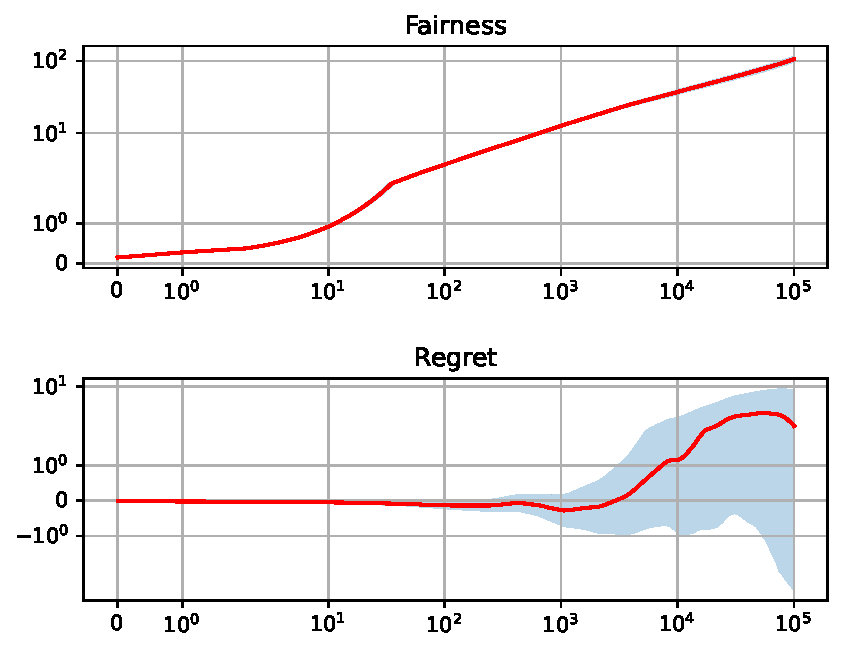
\includegraphics[width=0.8\textwidth]{../code/figures/mab_Greedy.pdf}
% 	\caption{Fair allocation and base bandit based on Greedy}
% 	\label{fig:}
% \end{figure}


% \begin{figure}[H]
% \centering
% 	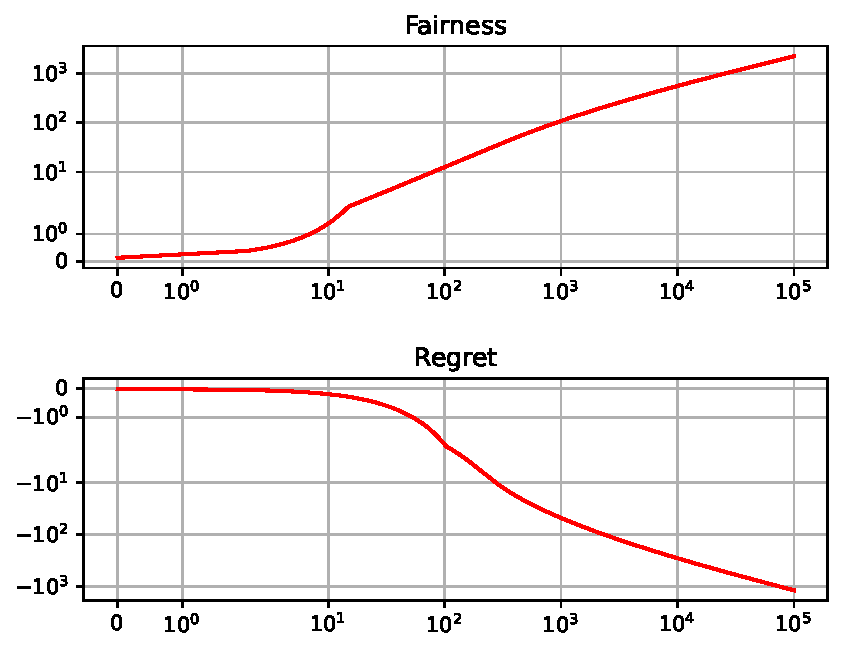
\includegraphics[width=0.8\textwidth]{../code/figures/mab_UCB.pdf}
% 	\caption{Fair allocation and base bandit based on UCB}
% 	\label{fig:}
% \end{figure}


% \begin{figure}[H]
% \centering
% 	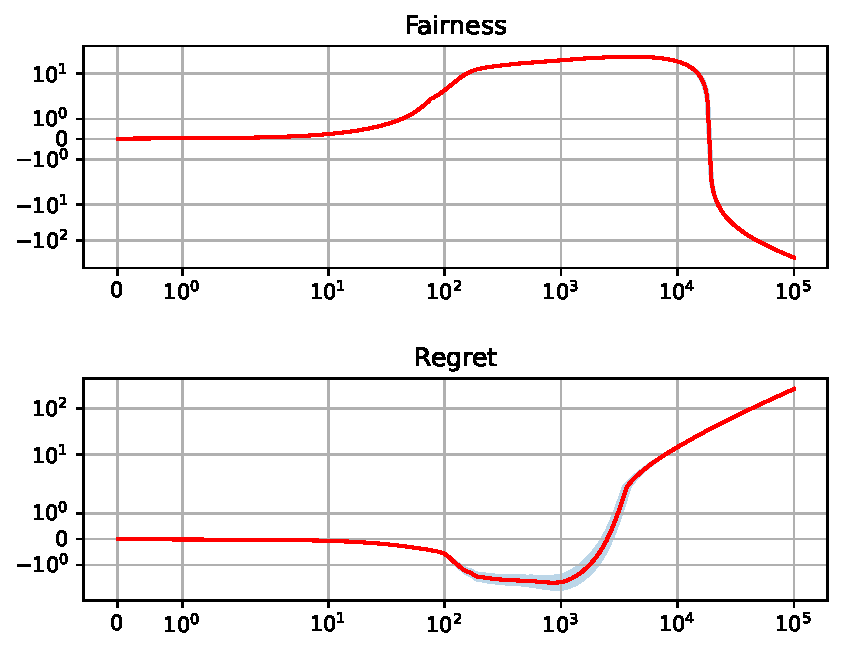
\includegraphics[width=0.8\textwidth]{../code/figures/mab_LCB.pdf}
% 	\caption{Fair allocation and base bandit based on LCB \hr{I believe this wierd behavior is because it takes long to find the correct arm, using Greedy or UCB for the base bandit should correct that}}
% 	\label{fig:}
% \end{figure}

\subsubsection{Greedy for base bandit, different fair allocations}

\subsubsection{UCB for base bandit, different fair allocations}

\subsection{Fair regret}

Consider Fair-MAB with any allocation. We first propose a generic upper bound that works under the three allocations that we proposed. We recall that we assume that $\max_j \mu_j \leq \mu^+$ for a known constant $\mu^+$, and that the problem is feasible so $\forall j \in [K], \wh q_{j,t}  \geq \alpha_j$ for some $\alpha_j>0$. For a time step $t$, consider the event \[\cG_t=\left\{ \forall k \in [K]\;:\; \mu_k \in [\LCB_{k, t}, \UCB_{k, t}], N_k(t)\geq \frac{\alpha_kt}{2}, \sum\frac{\lambda_j}{\wt \mu_{j,t}} \leq 1 \right\}\;,\]
 where we ommit the confidence levels in the notation for simplicity, but we will fix them later as a function of $t$. Consider an arm $k$, we want to upper bound $\cV_T^k \coloneqq \bE\left[\sum_{t=1}^T \left(\lambda_k-p_{k,t} \mu_k \right)\right]$.
 
We first write that 
\begin{align*}
\cV_T^k &\leq \bE\left[\sum_{t=1}^T \left(\lambda_k-p_{k, t} \mu_k \right)\right] \\
&
\leq  \underbrace{\bE\left[\sum_{t=1}^T \left(\lambda_k-\wh q_{k,t} \mu_k \right) \ind(\cG_t)\right]}_{V_1} + \underbrace{\bE\left[\sum_{t=1}^T \left(\lambda_k-p_{k, t} \mu_k \right) \ind(\bar \cG_t)\right]}_{V_2} \;. \\
\end{align*}


\paragraph{Upper bounding $V_1$} We first re-write $V_1$ as a function of $\wt \mu_{k, t}$ under $\cG_t$, 
\begin{align*}
V_1 & = \bE\left[\sum_{t=1}^T \left(\lambda_k- \frac{\lambda_k}{\wt \mu_{k, t}} \mu_k \right) \ind(\cG_t)\right] \\
& = \lambda_k \bE\left[\sum_{t=1}^T \left(\frac{\wt \mu_{k,t}-\mu_k}{\wt \mu_{k,t}}\right) \ind(\cG_t)\right]\;.
\end{align*}

Then, we remark that for the LCB allocation it simply holds that $V_1\leq 0$ since $\mu_k\geq \wt \mu_{k,t}$. Let us now consider the UCB allocation, under $\cG_t$ the term inside the expectation is non-negative and satisfies 
\[\frac{\wt \mu_{k,t}^{\UCB}-\mu_k}{\wt \mu_{k,t}^{\UCB}} \leq \frac{\UCB_{k,t}-\mu_k}{\mu_k} \leq \frac{\UCB_{k,t}-\LCB_{k, t}}{\mu_k} \;. \]
Furthermore, this bound also holds for the greedy allocation since the empirical mean also belong to the confidence interval. For these two allocations we thus obtain a bound that depend on the design of the confidence interval. 

We can give a more precise upper bound with the explicit form of the confidence interval. To provide a precise example, let us assume that the distributions are supported on $[0,1]$. For any $\delta>0$, Hoeffding's inequality states that 
\[\bP\left(|\wh \mu_{k, n}-\mu_k|\geq \delta \right)\leq 2e^{-2n\delta^2}\;, \]
so we can define for instance $\LCB_{k,t} = \wh \mu_k(t) - \sqrt{\frac{C\log(t)}{N_k(t)}} $ and $\UCB_{k,t} = \wh \mu_k(t) + \sqrt{\frac{C\log(t)}{N_k(t)}}$ for some $C>0$ to obtain a confidence level as a power of $t^{-1}$. Indeed, if holds that 
\begin{align*} \bP\left(|\wh \mu_k(t)- \mu_k|\geq \sqrt{\frac{C\log(t)}{N_k(t)}}, N_k(t)\geq \frac{\alpha_k t}{2} \right)&\leq \sum_{n=\frac{\alpha_k t}{2}}^t \bP\left(|\wh \mu_{k, n}- \mu_k|\geq \sqrt{\frac{C\log(t)}{n}}\right)  \\
&\leq 2 \sum_{n=\frac{\alpha_k t}{2}}^t t^{-2C}\leq \frac{2}{t^{2C-1}} \;,
\end{align*}

that we will use later in our analysis. For now, we simply use that this tuning ensures that \[\UCB_{k,t}-\LCB_{k, t} = 2\sqrt{\frac{C\log(t)}{N_k(t)}} \leq 2\sqrt{\frac{C\log(t)}{\alpha_k t}} \;, \]
again using that under $\cG_t$ it holds that $N_k(t)\geq \frac{\alpha_k}{2}t$. Plugging this into the upper bound on $V_1$, we obtain for the Greedy and UCB allocations that 

\[V_1 \leq \frac{\lambda_k}{\mu_k} \sum_{t=1}^T 2 \sqrt{\frac{C\log(t)}{\alpha_k t}} \leq 2\frac{\lambda_k}{\mu_k}\sqrt{\frac{CT\log(T)}{\alpha_k}}\;. \] 


\paragraph{Upper bounding $V_2$} A union bound provides that 
\begin{align*}
V_2 & \leq \lambda_k \sum_{j=1}^K \sum_{t=1}^T \bP(\mu_j \notin [\LCB_{j, t}, \UCB_{j, t}])  + \lambda_k \sum_{j=1}^K \sum_{t=1}^T\bP\left(N_j(t)\leq \frac{\alpha_j}{2}\right) \\
&+ \sum_{t=1}^T \bE\left[(\lambda_k - \wh q_{k,t}\mu_k)\ind\left(\forall j \in [K]; \mu_j \in [\LCB_{j, t}, \UCB_{j, t}], N_j(t)\geq \frac{\alpha_j}{2}t,  \sum_j \wh q_{j,t} \geq 1\right)\right] 
\end{align*}
 
First, we remark $\sum_{j=1}^K \sum_{t=1}^T \bP(\mu_j \notin [\LCB_{j, t}, \UCB_{j, t}])$ only depend on the confidence level of our LCB/UCBs. To make the sum converge we can for instance choose $\delta_t = 1/t^2$ and the first term of the upper bound of $V_2$ becomes $\cO(\lambda_k)$. With the Hoeffding's bound presented above, this condition is satisfied for $C=\frac{3}{2}$.

The second term can be upper bounded using that, at each time step $t$, the sampling probability of each arm $j$ is at least $\alpha_j$. Hence, $N_j(t)$ is stochastically dominated by a sum of i.i.d. Bernoulli random variables with probability $\alpha_j$, which leads to 
\begin{align*}
\sum_{j=1}^K \sum_{t=1}^T\bP\left(N_j(t)\leq \frac{\alpha_j}{2}\right) \leq \sum_{j=1}^K \sum_{t=1}^T e^{-t \kl\left(\frac{\alpha_j}{2}, \alpha_j\right)} \leq  \sum_{j=1}^K   \frac{1}{\kl\left(\frac{\alpha_j}{2}, \alpha_j\right)} \leq \sum_{j=1}^K\frac{2}{\alpha_j^2}\;,
\end{align*}
where $\kl$ denotes the Bernoulli KL-divergence. We get the intermediate result 

\[V_2 \leq \sum_{j=1}^K   \frac{1}{\kl\left(\frac{\alpha_j}{2}, \alpha_j\right)} + V_2'+ \cO(\lambda_k),  \]

with $V_2'=\sum_{t=1}^T \bE\left[(\lambda_k - \wh q_{k,t}\mu_k)\ind\left(\forall j \in [K]; \mu_j \in [\LCB_{j, t}, \UCB_{j, t}], N_j(t)\geq \frac{\alpha_j}{2}t, \sum_j \wh q_{j,t} \geq 1\right)\right]$.

We now upper bound the term $V_2'$, that depends on the choice of $\wt \mu_{k,t}$. Among our three allocations, the simplest case is UCB. Indeed, when all $(\mu_k)$ belong to their confidence bands it simply holds that  \[\sum_{j=1}^K \frac{\lambda_j}{\wt \mu_{j,t}^{\UCB}} \leq \sum_{j=1}^K \frac{\lambda_j}{ \UCB_{j,t}} \leq \sum_{j=1}^K \frac{\lambda_j}{ \mu_j}\;,\] so the UCB allocation is feasible and it directly holds that $V_2=\cO(\lambda_k)$ since the second term of its upper bound is in fact $0$.

If the allocation is LCB or greedy, the analysis is more involved, and we propose different paths depending  on the value of the feasibility gap $\rho_\lambda$: if $\rho_\lambda$ is positive, after some time normalization will not be needed with high probability, while if $\rho_\lambda=0$ (or is very small) it is likely to be needed for a long time.

By design the confidence bands also satisfy that $\wh \mu_j \in [\LCB_{j, t}, \UCB_{j, t}]$, it holds for all allocations that $\wt \mu_{j, t}\geq \mu_j- B_{j, t}$, with $B_{j,t} = \UCB_{j, t} - \LCB_{j, t}$. So, 

\begin{align*}
\sum_{j=1}^K \frac{\lambda_j}{\wt \mu_{j, t}} \leq \sum_{j=1}^K \frac{\lambda_j}{\mu_j - B_{j, t}} &= \sum_{j=1}^K \frac{\lambda_j}{\mu_j}\left(\frac{1}{1-\frac{B_{j, t}}{\mu_j}}\right) \\ &= \sum_{j=1}^K \frac{\lambda_j}{\mu_j} + \sum_{j=1}^K \frac{\lambda_j}{\mu_j}\times \frac{B_{j, t}}{1 - \frac{B_{j, t}}{\mu_j}} \\
& = 1-\rho_\lambda +\sum_{j=1}^K \frac{\lambda_j}{\mu_j}\times \frac{\frac{B_{j, t}}{\mu_j}}{1 - \frac{B_{j, t}}{\mu_j}}   \\
& \leq (1-\rho_\lambda)\left(1+ \max_{j\in[K]}\frac{\frac{B_{j, t}}{\mu_j}}{1 - \frac{B_{j, t}}{\mu_j}} \right) \;.  \\
\end{align*}

We now remember that we use this result under the event that each arm $j$ satisfies $N_j(t)\geq \alpha_j \frac{t}{2}$. The upper bound is increasing with $B_{j,t }$, which is itself upper bounded by its value for $N_j(t)= \alpha_j \frac{t}{2}$. With a Hoeffding's bound, the upper bound hence becomes 
\[\sum_{j=1}^K \frac{\lambda_j}{\wt \mu_{j, t}} \leq (1-\rho_\lambda)\left(1+ \max_{j\in[K]}\frac{\frac{2}{\mu_j}\sqrt{\frac{C\log(t)}{\alpha_j t}}}{1-\frac{2}{\mu_j}\sqrt{\frac{C\log(t)}{\alpha_j t}}} \right),\]
which is valid when $t$ is large enough so that the denominator is positive. We thus define the time \[t_\lambda(\CB)= \inf\left\{t \in \N: \; \max_j \frac{B_{j,t}}{\mu_j}\leq \frac{1}{2} | N_j(t)\geq \frac{\alpha_j}{2}t \right\}\;,\] so that for $t\geq t_\lambda$ we have that $B_{j,t}\leq \mu_j/2$. We can verify that $t_\lambda=\cO\left(\max_j\frac{1}{\alpha_j\mu_j^2}\log\left(\frac{1}{\alpha_j\mu_j^2}\right)\right)$.

Similarly, we can define the following deterministic time
\[t_\lambda'(\CB)= \inf\left\{t \in \N: \; \max_j \frac{B_{j,t}}{\mu_j}\leq \frac{\rho_\lambda}{2} | N_j(t)\geq \frac{\alpha_j}{2}t \right\}\;,\] so that for $t\geq \max\{t_\lambda(\CB), t_\lambda'(\CB)\}$ we have that $\sum_{j=1}^K \frac{\lambda_j}{\wt \mu_{j, t}} \leq 1$. We can also verify that $t_\lambda'(\CB)=\cO\left(\max_j\frac{1}{\alpha_j(\rho_\lambda \mu_j)^2}\log\left(\frac{1}{\alpha_j(\rho_\lambda \mu_j)^2}\right)\right)$, and is then scaling as $\rho_\lambda^{-2}$ if $\rho_\lambda>0$ and is infinite otherwise.

In the case where $\rho_\lambda>0$ we can simply write that \[V_2' \leq \max\{t_\lambda(\CB), t_\lambda'(\CB)\}= \cO\left(\max_j\frac{1}{\alpha_j(\rho_\lambda\mu_j)^2}\log\left(\frac{1}{\alpha_j(\rho_\lambda\mu_j)^2}\right)\right).\]

In the case where $\rho_\lambda=0$, we provide the following upper bound when $t \geq t_\lambda(\CB)$ and all the events considered in $V_2'$ hold, 
\begin{align*}
\lambda_k - \wh q_{k,t} \mu_k & = \lambda_k \left(1- \frac{\mu_k}{\wt \mu_{k, t}\left(1+2\max_j \frac{B_{j,t}}{\mu_j}\right)}\right) \\ 
& \leq \lambda_k \left(\frac{\wt \mu_{k,t}- \mu_k}{\wt \mu_{k, t}\left(1+2\max_j \frac{B_{j,t}}{\mu_j}\right)} +2\max_j \frac{B_{j,t}}{\mu_j} \right) \;.
\end{align*} 
For the LCB allocation the first term is negative under the events considered, while for the greedy allocation it can be upper bounded by $\frac{B_{k,t}}{\mu_k}$ just like $V_1$. The second term brings a $2\sum_{t=1}^T \max_j B_{j,t}/\mu_j$ to the regret, which gives $4\lambda_k\sqrt{\frac{C\log(T)T}{\min_{j \in [K]} (\alpha_j\mu_j^2)}}$ for the Hoeffding's bounds.

If we combine our two results, it holds for the greedy allocation that
\[ V_2' \leq \lambda_k\left(t_\lambda(\CB) + \left(t_\lambda'(\CB)-t_\lambda(\CB) \vee  \sum_{t=1}^T \left(\frac{B_{k,t}}{\mu_k}+2\max_{j\in[K]}B_{j,t}\right)\ind\left(N_k(t)\geq \alpha_k\frac{t}{2}\right) \right)\right) \;,   \]

which is asymptotically constant if $\rho_\lambda>0$ and scales in $\lambda_k \sqrt{\frac{T\log(T)}{\min (\alpha_j \mu_j^2 )}}$ if $\rho_\lambda=0$. Quite similarly, for the LCB allocation we obtain that
\[ V_2' \leq \lambda_k\left(t_\lambda(\CB) + \left(t_\lambda'(\CB)-t_\lambda(\CB) \vee 2\sum_{t=1}^T \max_{j\in[K]}B_{j,t}\ind\left(N_k(t)\geq \alpha_k\frac{t}{2}\right) \right)\right)  \;.   \]

\paragraph{Summary} We summarize our results, applying them for distributions with bounded supports and confidence intervals using Hoeffding's inequality. This way, we can exhibit a precise scaling in all the components of the problem. By upper bounding $V_1$ and $V_2$ we proved the following results when $\rho_\lambda>0$. 

For the LCB allocation,
\hr{$V_1$ decreases linearly while $V_2$ is constant, this means the fairness regret decreases linearly, we obtain negative fairness regret for LCB which is consistant with the simulations.
}

	\[\cV_T \leq \left(\max_{k \in K}\lambda_k\right) \left( K \sum_{t=1}^{+\infty} \frac{1}{t^2} + \sum_{j=2}^K\frac{1}{\kl\left(\frac{\alpha_j}{2}, \alpha_j\right)} + \cO\left(\max_j\frac{2}{\alpha_j(\rho_\lambda \mu_j)^2}\log\left(\frac{2}{\alpha_j(\rho_\lambda \mu_j)^2}\right)\right)\right) \;, \]
so the fair regret is upper bounded by a problem-dependent constant. 

For the greedy allocation, 
	\begin{align*} \cV_T \leq \max_{k\in K} &\left(\frac{2\lambda_k}{\mu_k}\sqrt{\frac{C T \log(T)}{\alpha_k}}+ \lambda_k\left(K \sum_{t=1}^{+\infty} \frac{1}{t^2} + \sum_{j=2}^K\frac{1}{\kl\left(\frac{\alpha_j}{2}, \alpha_j\right)} \right.\right. \\
	& \left.\left. + \cO\left(\max_j\frac{2}{\alpha_j(\rho_\lambda \mu_j)^2}\log\left(\frac{2}{\alpha_j(\rho_\lambda \mu_j)^2}\right)\right)\right)\right) \;. \end{align*}
\hr{I think this is shoting ourselves in the foot, if we cannot prove that Greedy has better fairness than UCB then let's remove Greedy.}

And for the UCB allocation, 
		\begin{align*} \cV_T \leq \max_{k\in K} &\left(\frac{2\lambda_k}{\mu_k}\sqrt{\frac{C T \log(T)}{\alpha_k}}+ \lambda_k\left(K \sum_{t=1}^{+\infty} \frac{1}{t^2} + \sum_{j=2}^K\frac{1}{\kl\left(\frac{\alpha_j}{2}, \alpha_j\right)}\right)\right) \;. \end{align*}
Furthermore, when $\rho_\lambda$ is small or $0$ the term in $\rho_\lambda^{-2}$ can be replaced by the upper bounds on $V_2'$ presented above, scaling (if we consider $T$ only) in $\sqrt{T\log(T)}$. The fact that it is possible in some cases to get a problem-dependent constant upper bound for the LCB allocation proves that the Fair Bandit equipped with this allocation will satisfy the fairness constraint faster than with the other approaches on average. On the other hand, UCB and Greedy both provide a bound of order $\cO(\sqrt{T\log(T)})$ in all cases. However, the second-order term of UCB is better since it does not depend on the feasibility gap. This has another advantage, which is that the upper bound for UCB do not depend on $\mu_k$ (since $\lambda_k/\mu_k \leq 1$) but only on $(\alpha_j)_{j \in [K]}$ (more precisely in $\max_j \alpha_j^{-2}$).

\hr{Currently, the bound does not behave well when $\lambda_{k} \to 0$, since this implies $\alpha_{k} \to 0$. This should not happen since all allocations should be fair when $\lambda_k \to 0$.}

\subsection{Bandit regret}

We know upper bound the bandit regret for the three instances of Fair MAB that we considered. Similarly to what we did in previous section, we consider the following good event
 \[\cG_t=\left\{ \forall k \in [K]\;:\; \mu_k \in [\LCB_{k, t}, \UCB_{k, t}], N_k(t)\geq \frac{\alpha_k t}{2} \right\}\;.\]
 The main difference is that here it is not necessary to check the value of $\sum_j \frac{\lambda_j}{\wt \mu_{j,t}}$, since in any case it holds that $p_{k,t}\leq \frac{\lambda_k}{\wt \mu_{k,t}}$. This will simplify the analysis of $\bP(\bar \cG_t)$ compared to previous section.


We denote by $\cR_{T,k}$ the contribution of a sub-optimal arm $k$ to the bandit regret, and first write that 
\begin{align*}
\cR_{T,k} &= \bE\left[\sum_{t=1}^T (p_{k,t} - p^\star_k)(\ind(\cG_t)+\ind(\bar \cG_t))\right]\Delta_k \\
& \leq \sum_{t=1}^T (1-p_k^\star) \bP(\bar \cG_t) + \bE\left[\sum_{t=1}^T (p_{k,t} - p_k^\star)\ind(\cG_t)\right] \Delta_k \;.
\end{align*}

We can use our results from previous section, obtaining that for all allocations 
\[\sum_{t=1}^T \bP(\bar \cG_t) \leq K \sum_{t=1}^{+\infty} t\delta_t + \sum_{j=2}^K\frac{1}{\kl\left(\frac{\alpha_j}{2}, \alpha_j\right)}\;, \]
where $\delta_t$ is the confidence level chosen for each interval $[\LCB_{k,t}, \UCB_{k,t}]$. We can hence focus on upper bounding $\cS_{T, k} \coloneqq \bE\left[\sum_{t=1}^T (p_{k,t} - p_k^\star)\ind(\cG_t)\right]$. 

Using Equation~\eqref{eq::sampling_prob}, we obtain that 
\begin{align*}\cS_{T,k} &= \bE\left[\sum_{t=1}^T (\wh q_{k, t} + (1-\sum_j \wh q_{j, t}) \ind(k_t=k) - p_k^\star)\ind(\cG_t)\right] \\
& \leq   \underbrace{\bE\left[\sum_{t=1}^T (\wh q_{k, t}-p_k^\star) \ind(\cG_t)\right]}_{\cO_{ T,k}} + \underbrace{\bE\left[\sum_{t=1}^T (1-\sum_j \wh q_{j, t}) \ind(k_t=k)\ind(\cG_t)\right]}_{\cB_{T,k}} \;.
\end{align*}

This upper bound separates the regret due to the allocation ($\cO_{T,k}$) and the regret due to the base bandit ($\cB_{T,k}$). We now further upper bound these two terms separately.

\paragraph{Upper bounding $\cO_{T, k}$} The regret due to the allocation can be upper bounded very similarly as the term $V_1$ of the fair regret (see previous section). Indeed, we can re-write $\cO_{T,k}$ as 
\[\cO_{T,k} =\bE\left[\sum_{t=1}^T \frac{\lambda_k}{\mu_k}\left(\frac{\mu_k-\wt \mu_{k, t}}{\wt \mu_{k, t}} \wedge 1 \right) \ind(\cG_t)\right] \;.  \]

Under $\cG_T$, the UCB allocation ensures that $\wt \mu_{k, t}\geq \mu_k$, so $\cO_{T,k}=0$. 
\hr{Actually, this is where we see negative regret appear for UCB since it will be negative linear regret against positive square root}

For the two other policies it is easy to verify that 
\[ \cO_{T,k} \leq \bE\left[\sum_{t=1}^T \frac{\lambda_k}{\mu_k}\left(\frac{\UCB_{k, t}- \LCB_{k, t}}{\LCB_{k, t}}\wedge 1\right) \ind(\cG_t)\right].\]
We reuse $t_\lambda(\CB)$ from the previous section (for $t\geq t_\lambda(\CB)$, we have $\LCB_{k,t}\geq \frac{\mu_k}{2}$ if $N_k(t)\geq \frac{\alpha_k t}{2}$). It holds directly that 
\[\cO_{T,k} \leq \frac{\lambda_k}{\mu_k} \left(t_\lambda(\CB) + \frac{2}{\mu_k}\bE\left[\sum_{t=t_k}^T (\UCB_{k, t}- \LCB_{k, t}) \ind(\cG_T)\right] \right) \;. \]

As before, we can be more specific for Hoeffding's bounds, and obtain (see previous section for details) that
\[ \cO_{T,k} \leq 2\frac{p_k^\star}{\mu_k}\sqrt{\frac{T\log(T)}{\alpha_k}} + \cO\left(\frac{\lambda_k}{\alpha_k \mu_k^3}\log\left(\frac{4}{\alpha_k \mu_k^2}\right)\right)  \;. \]


\paragraph{Upper bounding $\cB_{T, k}$} \textcolor{blue}{I continue the proof for a UCB algorithm, the proof is actually straightforward for optimistic algorithms since the best arm is represented by its UCB. For other policies the analysis would be more involved: we would need to make sure that the best arm is sampled enough to have a good mean, so that the algorithm is well-performing. We would surely need for instance that the probability of playing the bandit is large enough (e.g larger than $\rho_\lambda/2$), and we would get in that case a factor $2/\rho_\lambda$ in front of the upper bound of the second-order term of the standard bandit regret.\\
Adapt the message in the main text depending on what we find.}

\hr{Ok here, I believe we should actually use UCB to choose the arm (depending on the values of $\lambda$) so that we always have a good behavior for the allocation of the arm.
Then, we can either choose UCB or LCB to focus on fairness or regret}

First, under $\cG_t$ we can provide a deterministic upper bound of $1-\sum_j \wh q_{j,t} $. Indeed,
\begin{align*}
1-\sum_j \wh q_{j,t} & \leq 1 - \sum_j \frac{\lambda_j}{\UCB_{j,t}} \\
& \leq 1- \sum_j \frac{\lambda_j}{\mu_j + B_{j,t}} \\
& \leq 1- \left(\sum_j \frac{\lambda_j}{\mu_j}\left(1- \frac{B_{j, t}/\mu_j}{1+B_{j,t}/\mu_j}\right) \right) \\
& \leq \rho_\lambda + \sum_j \frac{\lambda_j}{\mu_j^2} B_{j,t}\\
&\leq \rho_\lambda + (1-\rho_\lambda)\max_{j \in[K]} \frac{B_{j,t}}{\mu_j} \to \rho_\lambda \;.
\end{align*}

Hence, (to avoid painful term-by-term upper bounds involving $\max_{j \in[K]} \frac{B_{j,t}}{\mu_j}$) we state that \[\bE\left[\sum_{t=1}^T (1-\sum_j \wh q_{j, t}) \ind(k_t=k)\ind(\cG_t)\right] = \rho_\lambda \bE\left[\sum_{t=1}^T \ind(k_t=k)\ind(\cG_t)\right] + o\left(\bE\left[\sum_{t=1}^T \ind(k_t=k)\ind(\cG_t)\right]\right)\;, \]
so we now focus on upper bounding the term $\bE\left[\sum_{t=1}^T \ind(k_t=k)\ind(\cG_t)\right]$. We consider a UCB base bandit, that chooses $k_t = \argmax{} \UCB_{k, t}$. Even if the algorithm uses observations that were not necessarily collecting because of its policy, the analysis can be fully conducted following the proof steps of any standard analysis of a UCB policy.  We first write that

\begin{align*}
\bE\left[\sum_{t=1}^T \ind(A_{t+1}=k, \UCB_{k, t}\geq \max_j \UCB_{j, t}, \cG_t)\right] & \leq \bE\left[\sum_{t=1}^T \ind(A_{t+1}=k, \UCB_{k, t}\geq \UCB_{1, t}, \cG_t)\right] \\
& \leq \bE\left[\sum_{t=1}^T \ind(A_{t+1}=k, \UCB_{k, t}\geq \mu_1)\right] \;. \end{align*}

Classically, we then use that for $N_k(t)\geq \frac{2C}{\Delta_k^2} \log(t)$ we have that $\UCB_{k, t}\geq \mu_1 \Rightarrow \wh \mu_{k, t} \geq \mu_k + \frac{\Delta_k}{2}$, so we can obtain that 

\begin{align*}
\bE\left[\sum_{t=1}^T \ind(A_{t+1}=k, \UCB_{k, t}\geq \mu_1)\right] &\leq \frac{2C}{\Delta_k^2} \log(T) + \sum_{n=\frac{2C}{\Delta_k^2} \log(T)}^T \bP\left(\wh \mu_{k, n}\geq \mu_k + \frac{\Delta_k}{2}\right) \\
& \leq \frac{2C}{\Delta_k^2} \log(T) + \frac{2}{\Delta_k^2} \;.
\end{align*}

Note that this bound holds even if $\lambda_k=0$, which is expected since it is the standard upper bound of the regret of \texttt{UCB1}. We thus obtain the folklore results of $\cO(\log(T))$ problem-dependent bound and $\cO(\sqrt{T\log(T)})$ worst-case bound.

Interestingly, if $\lambda_k>0$ we can provide an alternative upper bound, that provides a constant problem-dependent upper bound. Indeed, we recall that under $\cG_t$ it holds that $N_k(t)\geq \alpha_k \frac{t}{2}$, and so the first term can in fact be replaced by $\frac{2C}{\Delta_k^2}\log(T)\wedge t_k$, where $t_k$ is defined as follows,
\[t_k = \inf\{t\in \N: \; \frac{\alpha_k}{2}t\leq \frac{2C}{\Delta_k^2} \log(t) \}= \cO\left(\frac{4C}{\alpha_k \Delta_k^2}\log\left(\frac{4C}{\alpha_k\Delta_k^2}\right)\right)\;.\]

Hence, in all generality we finally obtain that 
\begin{align*}
\bE\left[\sum_{t=1}^T \ind(A_{t+1}=k, \UCB_{k, t}\geq \mu_1, \cG_t)\right] &\leq t_k \wedge  \frac{2C}{\Delta_k^2}\log(T) + \frac{2}{\Delta_k^2} \;.
\end{align*}

Hence, if $\lambda_k>0$, the base bandit only adds a problem-dependent constant to $\cS_{T,k}$, however the worst-case bound remains the one of UCB, namely $\cO(\sqrt{KT\log(T)})$.

\paragraph{Summary} We recall that $\cR_{T,k}\leq \sum_{t=1}^T \bP(\bar \cG_t)+\cO_{T, k}+ \cB_{T,k}$, where the terms are defined above. 
\begin{itemize}
	\item For the UCB allocation, it holds that 
	\[\cR_{T,k}^\text{\UCB} \leq \sum_{k: \Delta_k>0}\left((1-p_k^\star)\Delta_k \left(K \sum_{t=1}^{+\infty} t\delta_t + \sum_{j=2}^K\frac{1}{\kl\left(\frac{\alpha_j}{2}, \alpha_j\right)}\right) + (t_k\Delta_k) \wedge  \frac{2C}{\Delta_k}\log(T) + \frac{2}{\Delta_k} \right) \;. \]
	\item For the LCB and greedy allocations it holds that 
	\[ \cR_{T,k}^{\texttt{Greedy}/\LCB} \leq \cR_{T,k}^\UCB + \sum_{k:\Delta_k>0} 2\frac{p_k^\star}{\mu_k}\sqrt{\frac{T\log(T)}{\alpha_k}} \Delta_k
	\]
\end{itemize}



\begin{remark}[Negative problem-dependent bound] 
	
	It is easy to see that if we take for instance $2C$ in the confidence bound then the only change in the above analysis are (1) the logarithmic term is doubled, (2) $p_{k, t}-p_k^\star\leq \frac{\lambda_k}{\mu_k+\sqrt{C\frac{\log(t)}{N_k(t)}}}-\frac{\lambda_k}{\mu_k}\leq \frac{\lambda_k}{\mu_k+\sqrt{\frac{C_\alpha}{t}}}-\frac{\lambda_k}{\mu_k}$ for $C_\alpha=\frac{2C}{\alpha_k}$. We obtain that
	\[\bE\left[\sum_{t=1}^T(p_{k,t}-p_k^\star)\ind(\cG_t)\right] \leq \sum_{t=1}^T \frac{\lambda_k}{\mu_k+\sqrt{\frac{C_\alpha}{t}}}-\frac{\lambda_k}{\mu_k} = -\Omega\left(-\frac{\lambda_k}{\mu_k^2}\sqrt{C_\alpha T}\right)\;,
	\]
	
	If we again consider the highly probable event $N_k(t)\geq \alpha_k t/2$, we then have that the term that we upper bounded by $0$ now becomes $-\Omega(\sqrt{T})$. This gives a negative problem-dependent regret asymptotically.
\end{remark}


\begin{remark}[Scaling of the bounds in $\alpha_k$] 
	This is maybe the major weakness in our results, but getting finer bounds may require a much more involved analysis. It could be avoided by using a forced exploration, but this would have an impact on other terms, resulting in a different (larger) scaling in $T$. In particular we would have $T^{3/4}$ if we force $p_{k,t}\geq 1/\sqrt{t}$, multiplicative $\log(t)^{k/2}$ if $p_{k,t}\geq (\log(t))^{-k}$, \dots). 
\end{remark}

\paragraph{Conclusion of this part} There is no overall winner among the three allocations: LCB is good for the fair regret while UCB is good if minimizing the bandit regret is preferred; while greedy performs similarly as the worst of the two in both cases, up to a factor $1/2$ in the first order term (we did not precise this). However, it is not exactly symmetric, since UCB guarantees with high probability that the proposition of the allocation is feasible without normalization, which has an impact on the fair regret.


\subsection{Unfeasible case}

\textcolor{blue}{This section was written before introducing the normalization directly in the algorithm, change this later. I think that the adaptation of the analysis would be straightforward,} \textcolor{red}{if we ensure a sample size guarantee with forced exploration, because we can no longer use $p_{k,t}\geq \lambda_k/(K\mu^+)$}. \textcolor{blue}{Of course, another constraint like $\sum \frac{\lambda_j}{\mu_j}\leq B$ for $B\geq 1$ would suffice (alternatively, $\min \frac{\mu_j}{\lambda_j}\geq a$ for some $a>0$).}

The only point that may be interesting is just that if we propose 
	\[ \wh q_{k, t} = \frac{\lambda_k}{\UCB_{k,t}} \left(\sum_{j \in [K]}\frac{\lambda_j}{\LCB_{j,t}}\wedge1 \right)^{-1} \;, \]
	we can still get a constant problem-dependent regret with a UCB allocation since we will have under $\cG_t$ that $\wh q_{k, t} \leq p_k^\star$.
	
\textcolor{blue}{In the future paper this may just be left as a remark.}

\subsection{Sufficient exploration without a upper bound on the means}

We may change the event $\cG_t$ so that it contains $\{\forall k \in [K],\forall s \leq t\;, \mu_k \in [\LCB_{k,s}, \UCB_{k,s}] \}$ instead of $\{\forall k \in [K], \mu_k \in [\LCB_{k,t}, \UCB_{k,t}] \}$. We just need to increase the radius (tuned with $C$) of the bounds to make this event high probability (one more union bound of $t$ terms in the upper bound of the converse event).
\textcolor{blue}{I've been too fast on this, it is impossible because $\sum_{t=1}^T \bP(\exists s: \mu_k \notin [\LCB_{k,s}, \UCB_{k,s}])\geq T \bP(\mu_k \notin [\LCB_{k,1}, \UCB_{k,1}])$. We need  to know $T$ if we want this to hold, and tune the confidence bounds with $\log(T)$. In that case we can have
\[\bE\left[\sum_{t=1}^T \ind(\exists s\in [t]: \mu_k \notin [\LCB_{k,s}, \UCB_{k,s}]) \right] \leq T \sum_{n=1}^T \bP(\mu_k \notin [\wh \LCB_{k,n}, \wh \UCB_{k,n}])\;, \]
where the last term involves the value of the bounds when the sample size is $n$ (when this is fixed there is no more dependency in $s$). Tuning the bounds to get a confidence $T^{-2}$ is sufficient in our analysis.
}
\textcolor{red}{We need to determine if we prefer the bounded means assumption and anytime algorithms, or knowing $T$ and no assumption on the means.}

\textcolor{blue}{Alternative that may work anytime: $\cG_t=\{\forall k \in [K], \mu_k \in [\LCB_{k,t}, \UCB_{k,t}] \}$, and consider $\sum_{t=1}^T\ind\left(\sum_{s=1}^t \ind(\bar \cG_s) \geq \frac{t}{2} \right)$. We can prove that this sum converges with Chernoff method, using that $\bP(\bar \cG_s)=\cO(s^{-2})$ for instance.}

Let us consider the UCB allocation so that there normalization was never needed when $\cG_t$ holds.

In that case, it holds that \[\forall k \in [K],\;\forall s \in [t],\; \wh q_{k,s} = \frac{\lambda_k}{\UCB_{k,s}} \geq \frac{\lambda_k}{\mu_k + 2 B_{k, s}} \;, \]

and recall that $B_{k,s}=\sqrt{\frac{C\log(s)}{N_k(s)}}$. Now, we can consider the probability of the event $\{N_k(t)\leq \frac{\lambda}{8\mu_k}t \}$ in this context. We remark that for any $s\in [t]$, if $N_k(s) \geq n_t \coloneqq \frac{C\log(t)}{4\mu_k^2}$ then $\wh q_{k,s}\geq \frac{\lambda_k}{2\mu_k}$. This means that if this sample size is achieved for $s\leq t$ small enough, the sampling probability is large enough for sufficient exploration of arm $k$. We propose the following upper bound, that builds on this idea, assuming that $t$ is large enough so that $n_t\leq  \frac{1}{2}\frac{\lambda_k}{\mu_k + 2\sqrt{C\log(t)}}t$

\begin{align*}
\bP\left(N_k(t)\leq \frac{\lambda}{8\mu_k}t\right) & \leq \bP\left(N_k(t)\leq \frac{\lambda}{8\mu_k}t, N_k(t/2)\geq n_t\right) + \bP\left(N_k(t)\leq \frac{\lambda}{8\mu_k}t, N_k(t/2)\leq n_t\right) \\
& \leq e^{-\frac{t}{2} \kl\left(\frac{\lambda_k}{4\mu_k}, \frac{\lambda_k}{2\mu_k}\right)} + \bP\left(N_k(t)\leq \frac{\lambda_k}{8\mu_k}t, N_k(t/2)\leq n_t\right) \\
&  \leq e^{-\frac{t}{2} \kl\left(\frac{\lambda_k}{4\mu_k}, \frac{\lambda_k}{2\mu_k}\right)} + \bP\left(N_k(t/2)\leq n_t\right) \;.
\end{align*}

The remaining term may look similar to the initial one, but there is a significant progress in the fact that we now compare to a logarithmic sample size, not a linear one. Indeed, it becomes sufficient to simply consider that under $\cG_t$ it holds that $\forall s \in [t/2] \wh q_{k,s}\geq \frac{\lambda_k}{\mu_k + 2 \sqrt{C\log(t/2)}}$, and so 
\begin{align*}
\bP\left(N_k(t/2)\leq n_t\right) & \leq e^{-\frac{t}{2}\kl\left(\frac{2 n_t}{t}, \frac{\lambda_k}{\mu_k + 2 \sqrt{C\log(t/2)}} \right)} \\
& \leq e^{-t \left(\frac{\lambda_k}{\mu_k + 2 \sqrt{C\log(t/2)}}- \frac{C\log(t)}{2\mu_k^2t}\right)^2}\;.
\end{align*}
We finally obtain a term that is asymptotically equivalent to $e^{-\lambda_k\frac{t}{4C\log(t/2)}}$, whose sum converges.

\textcolor{blue}{It this tight? Idk, this may be investigated. This is worse than what we obtained in the bounded case, but applicable in much broader settings.}

\subsection{Tentative stuff (probably garbage)}

\begin{lemma}
	In the case of Bernouilli reward, the Greedy estimate for $\widetilde{\mu_{k, t}}$ lead to a regret in $O(\log(T))$ (Proof does not work)
\end{lemma}
\begin{proof}
The total contribution to the regret can be written as:
\begin{align*}
\cR_{T,k} &= \bE\left[\sum_{t=1}^T \sum_{k=2}^K (p_{k,t} - p^\star_k)\right]\Delta_k \\
&= \sum_{t=1}^T \sum_{k=2}^K \bE\left[ (\wh q_{k, t} + (1-\sum_j \wh q_{j, t}) \ind(k_t=k) - p_k^\star) \right]\Delta_k \\
&= \sum_{t=1}^T \sum_{k=2}^K \left( \bE [ \wh q_{k, t} - p_k^\star]  + \bE [ (1-\sum_j \wh q_{j, t}) \ind(k_t=k) ] \right)\Delta_k \\
\end{align*}

Then we write 
\begin{align*}
	\bE [ \wh q_{k, t} - p_k^\star]  &= \bE [ \wh q_{k, t}] - p_k^\star \\
	&\leq  \bE [ \frac{\lambda_k}{\wh \mu_{k, t}} \ind(\mathcal{G}_{t})] + \bP(\bar \cG_t)  - p_k^\star \\
	&=  \bE [ \frac{\lambda_k}{ \mu_{k}(1 + \frac{\wh \mu_{k, t} - \mu_{k}}{\mu_{k}})} \ind(\mathcal{G}_{t})] + \bP(\bar \cG_t)  - \frac{\lambda_{k}}{\mu_{k}} \\
\end{align*}

Under $\mathcal{G}_{t}$, $ | \wh \mu_{k, t} - \mu_{k}| \leq \sqrt{\frac{C \log(t)}{N_k(t)}} \leq \sqrt{\frac{2 C \log(t)}{\alpha_{k} t}} $. Recall Taylor inequality: $|x| \leq a$, 
\[
\frac{1}{1 + x} \leq 1 - x + a^2	
\]
so we get:
\[
\frac{\lambda_k}{ \mu_{k}(1 + \frac{\wh \mu_{k, t} - \mu_{k}}{\mu_{k}})} \leq \frac{\lambda_{k}}{\mu_{k}}(1 - \frac{\wh \mu_{k, t} - \mu_{k}}{\mu_{k}} + \frac{2 C \log(t)}{\mu_{k}^2 \alpha_{k} t}) 
\]

Therefore:
\begin{align*}
	\bE [ \frac{\lambda_k}{ \mu_{k}(1 + \frac{\wh \mu_{k, t} - \mu_{k}}{\mu_{k}})} \ind(\mathcal{G}_{t})] &\leq  \bE [ \underbrace{\frac{\lambda_{k}}{\mu_{k}}(1 - \frac{\wh \mu_{k, t} - \mu_{k}}{\mu_{k}} + \frac{2 C \log(t)}{\mu_{k}^2 \alpha_{k} t})}_{> 0} \ind(\mathcal{G}_{t})] \\
&\leq  \bE [ \frac{\lambda_{k}}{\mu_{k}}(1 - \frac{\wh \mu_{k, t} - \mu_{k}}{\mu_{k}} + \frac{2 C \log(t)}{\mu_{k}^2 \alpha_{k} t})]
\end{align*}

So that we get:
\begin{align*}
	\bE [ \wh q_{k, t} - p_k^\star] &\leq  \frac{2 C \lambda_{k} \log(t)}{\mu_{k}^3 \alpha_{k} t}
\end{align*}




\end{proof}
%\section{Proof for Greedy}

Consider a randomized algorithm that samples an arm at time $t$ with probability $x_t \in \Delta_K$. We want an algorithm that satisfies the fairness constraint

\[\forall i \in [K]\;, \; \liminf \frac{1}{T} \bE\left[\sum_{t=1}^T x_{t,i} \mu_i \right] \geq \lambda_i \;,\]

i.e. all arms $i$ are guaranteed a minimum reward. If an algorithm satisfies this constraint, then we want to minimize the regret, that is defined by in the class of fair algorithms:

\[ \cR_T = \sum_{t=1}^T \bE\left[(x^\star - x_t)^\top\mu \right]\;, \]

where $x^\star$ is one of the (not unique if several arms are optimal) optimal allocation among those that satisfy the constraint. It is more illustrative to write the regret only in terms of the sub-optimal arm. Indeed, for any $i\in [K]$ it holds that $x_i = 1-\sum_{j \neq i } x_j$. Assuming w.l.o.g. that arm $1$ is among the best arms, we obtain that 

\begin{equation}\label{eq::regret}\cR_T =  \sum_{k=2}^K \bE\left[\sum_{t=1}^T (x_{t, i} - x^\star_i)\right] \Delta_k \;, \end{equation}

where $\Delta_k = \mu_k - \mu_1$. This expression is closer to usual formulations of the regret.

Our claim is that this problem can be solved simply by using a greedy algorithm. For that, we first analyze the possible values for $x^\star$. First, it is clear that \[ \mu_k < \mu_1 \Rightarrow x_k^\star = \frac{\lambda_k}{\mu_k} \;. \]

Note that the problem is feasible only if $\sum_{k=1}^{k}\frac{\lambda_i}{\mu_i} \leq  1$. after allocating their probability to sub-optimal arms, any $x^\star$ satisfying \[  \forall j > 1,   x_j^\star = \frac{\lambda_j}{\mu_j} \text{ and } x_1^{\star}  = 1 -\sum_{k: \mu_k<\mu_1} x_k^\star \]
Note that the problem is feasible only if $\sum_{k=1}^{K}\frac{\lambda_i}{\mu_i}\leq1$. After allocating their probability to sub-optimal arms, any $x^\star$ satisfying \[ \forall j: \mu_j =\mu_1\;, \; x_j^\star \geq \frac{\lambda_j}{\mu_j} \text{ and } \sum_{j: \mu_j=\mu_1} = 1 -\sum_{k: \mu_k<\mu_1} x_k^\star \]

is valid, and is the unique solution if $1$ is the only optimal arm or $\sum \frac{\lambda_j}{\mu_j}=1$.

\paragraph{Greedy algorithm} The greedy algorithm simply consists in using the optimal policy corresponding to the empirical estimates of the mean if it provides a feasible allocation. If it's not the case we simply propose uniform sampling. Hence, the steps of the algorithms are: 
\begin{enumerate}
	\item $\forall j$, compute $\wh \mu_j$.
	\item Check if $\sum_{j=1}^K \frac{\lambda_j}{\wh \mu_j} \leq  1$, i.e. if the greedy allocation if feasible.
	\item If yes, use $x_j=\frac{\lambda_j}{\wh \mu_j}$ for each empirically sub-optimal arm, make the probability sum to $1$ by adding the remaining mass on the best empirical arm $\star = \aargmax \wh \mu_j$ (choose at random if several).
\end{enumerate}


\subsection{Analysis}

\paragraph{Fairness constraint} Fix any arm $i \in [K]$. For any sequence of events $(E_t)_{t\in[T]}$ we obtain that 

\begin{align*} 
\frac{1}{T} \bE\left[\sum_{t=1}^T x_{t,i} \mu_i \right] \geq 
\frac{1}{T} \bE\left[\sum_{t=1}^T x_{t,i} \mu_i \ind(E_t) \right]\;.
\end{align*}

For the analysis of Greedy, we define $E_t = \{x_{t,i} \geq \frac{\lambda_i}{\mu_i}-\gamma_t, \sum_{i=1}^K \frac{\lambda_i}{\wh \mu_{t, i}}\leq 1 \}$, for a sequence of constants $(\gamma_t)_{t \in \N}$. If $E_t$ holds, then the greedy allocation is feasible (second event) and we have that 

\begin{align*}  
\frac{1}{T} \bE\left[\sum_{t=1}^T x_{t,i} \mu_i \ind(E_t) \right] &\geq \frac{1}{T} \bE\left[\sum_{t=1}^T (\lambda_i - \gamma_t \mu_i) \ind(E_t) \right] \\
& \geq  \lambda_i - \frac{1}{T} \sum_{t=1}^T \gamma_t \mu_i \bP(E_t) - \frac{1}{T} \sum_{t=1}^T \bP(\bar E_t) \\
& \geq  \lambda_i - \frac{\mu_i}{T} \sum_{t=1}^T \gamma_t - \frac{1}{T} \sum_{t=1}^T  \bP(\bar E_t)\;.
\end{align*}

From this result, we see that our objective will be to optimize $\gamma_t$ in order to make both terms small. We now upper bound $\bP(\bar E_t)$ by using the fact that $x_{t,i}\geq \alpha_i \coloneqq \min(\lambda_i, K^{-1})$ depending if the algorithm uses greedy or uniform allocation, and using that $\wh \mu_{t, i}\leq 1$. This ensures a number of samples at least of order $\alpha_i t$ for each arm $i$ at each time step $t$. Hence, we further upper bound 

\[\bP(\bar E_t) \leq \bP\left(\bar E_t, \forall j \in [K]:\; N_j(t)\geq \frac{\alpha_j}{2}t\right) + \bP\left(\bar E_t, \exists j \in [K]:\; N_j(t)\leq \frac{\alpha_j}{2}t\right) \;. \]  

We start by upper bounding the second term, 

\begin{align*}
\bP\left(\bar E_t, \exists j \in [K]:\; N_j(t) \leq  \frac{\alpha_j}{2}t\right) \leq \sum_{j=1}^K e^{-t \kl\left(\frac{\alpha_j}{2}, \alpha_j\right)} \leq \sum_{j=1}^K e^{-t \frac{\alpha_j^2}{4}} \;,
\end{align*}
\begin{equation}\label{eq::linearly_sampled}
\bP\left(\bar E_t, \exists j \in [K]:\; N_j(t) \leq  \frac{\alpha_j}{2}t\right) \leq \sum_{j=1}^K e^{-t \kl\left(\frac{\alpha_j}{2}, \alpha_j\right)} \;,
\end{equation}

where $\kl$ denotes the Bernoulli KL-divergence, and we used the fact that $N_j(t)$ stochastically dominates a sum of i.i.d. Bernoulli random variables with mean $\alpha_j$. We now consider the first term, in which all arms are linearly sampled.

For simplicity, we assume that $\rho \coloneqq 1- \sum_{i=1}^K \frac{\lambda_i}{\mu_i}>0$, hence the problem is in the interior of the ``feasible set''. 
Under this assumption, the greedy problem is feasible if for instance 
\[\frac{\lambda_i}{\wh \mu_i}\leq \frac{\lambda_i}{\mu_i}+ \frac{\rho}{K} \Rightarrow \wh \mu_i \geq \frac{1}{\frac{1}{\mu_i}+\frac{\rho}{K}}=\frac{\mu_i}{1+\frac{\rho \mu_i}{K}} = \mu_{i} - \underbrace{\frac{\mu_i \frac{\rho \mu_i}{K}}{1+\frac{\rho \mu_i}{K}}}_{\epsilon_{i, \rho }} ;.\]
so that $\overline{E}_t \implies \exists i \in [K], \hat{\mu}_{i} <  \mu_{i}  - \epsilon_{i, \rho}$.
The probability of this event can be easily controlled with usual union bounds and concentration inequalities as the arms are linearly sampled:
\begin{align*}
\bP( \overline{E}_{t}, \forall j \in [K]: N_j(t) \geq \frac{\alpha_j}{2}t ) &\leq \bE[\bP( \exists i \in [K],  \hat{\mu}_{i} <  \mu_{i}  - \epsilon_{i, \rho}  | N_i(t) \geq \alpha_{i}t) )]	 \\
&\leq \sum_{i=1}^K \exp(- \alpha_i \frac{t}{2} d(\mu_i - \epsilon_{i, \rho}, \mu_{i})) \leq \sum_{i=1}^K \exp(- \alpha_i t \epsilon_{i, \rho}^2))
\end{align*}
Finally, if the greedy allocation is feasible we use that
\[x_{t,i} \geq \frac{\lambda_i}{\mu_i} - \delta_t \Rightarrow \wh \mu_{t,i} \leq \frac{\mu_i}{1-\delta_t \mu_i} \coloneqq \mu_i + \epsilon_{i, \delta_t} \;, \]
which is again a large deviation of the empirical mean if $\delta_t$ is large enough. We have that $\epsilon_{i, \delta_t} \approx \delta_t \mu_i^2$, so it is easy to see that $\delta_t$ of the form \[\delta_t = \frac{1}{\mu_i^2} \times \sqrt{\frac{2\gamma \log(t)}{\alpha_i t}}\;,\] 
for some constant $\gamma$, will be enough to do what we want.
For simplicity, we assume that $\rho \coloneqq 1- \sum_{i=1}^K \frac{\lambda_i}{\mu_i}>0$, hence the problem is in the interior of the ``feasible set''. Under this assumption, the greedy allocation is feasible if for instance \[\frac{\lambda_i}{\wh \mu_{t, i}}\leq \frac{\lambda_i}{\mu_i}+ \frac{\rho}{K} \Rightarrow \wh \mu_{t, i} \geq \frac{1}{\frac{1}{\mu_i}+\frac{\rho}{\lambda_iK}}=\frac{\mu_i}{1+\frac{\rho \mu_i}{\lambda_i K}}\coloneqq \mu_i - \epsilon_{i, \rho}\;.\]

Some calculation provide that $\epsilon_{i, \rho}=\rho \frac{\mu_i^2}{\mu_i \rho + \lambda_i K}$. Using this result, and Hoeffding's inequality we obtain that 

\begin{align*}
\bP\left(\sum_{i=1}^K \frac{\lambda_i}{\wh \mu_{t, i}}\geq 1, \forall j \in [K]:\; N_j(t)\geq \frac{\alpha_j}{2}t\right) & \leq \sum_{j=1}^K \sum_{n=\alpha_j \frac{t}{2}}^t \bP\left(\wh \mu_{t,j} \leq \mu_j - \epsilon_{j, \rho}\right) \\
& \leq \sum_{j=1}^K \sum_{n=\alpha_j \frac{t}{2}}^t e^{-2n \epsilon_{j, \rho}^2} \;. \\
\end{align*}
So, we obtain that
\begin{equation}\label{eq::feasability_greedy}
\bP\left(\sum_{i=1}^K \frac{\lambda_i}{\wh \mu_{t, i}}\geq 1, \forall j \in [K]:\; N_j(t)\geq \frac{\alpha_j}{2}t\right) \leq \sum_{j=1}^K \frac{e^{-2\alpha_j \frac{t}{2} \epsilon_{j, \rho}^2}}{2\epsilon_{j, \rho}^2} \;.
\end{equation}

To complete the proof it remains to upper bound the term \[P_{t,i} \coloneqq \bP\left(x_{t,i}\leq \frac{\lambda_i}{\mu_i}-\gamma_t, \sum_{i=1}^K \frac{\lambda_i}{\wh \mu_{t, i}}\leq 1, \forall j \in [K]:\; N_j(t)\geq \frac{\alpha_j}{2}t\right) \;.\]

If the greedy allocation is feasible we use that
\[x_{t,i} \geq \frac{\lambda_i}{\mu_i} - \gamma_t \Rightarrow \wh \mu_{t,i} \leq \frac{\mu_i}{1-\gamma_t \mu_i} \coloneqq \mu_i + \epsilon_{i, t}' \;, \]
with $\epsilon_{i, t}'= \gamma_t \frac{\mu_i^2}{1-\gamma_t\mu_i}$. We can then use the same arguments as for the previous term, obtaining that 

\begin{align*}
P_{t,i} &\leq \sum_{n = \alpha_i \frac{t}{2}}^t \bP(\wh \mu_{n,i}\geq \mu_i + \epsilon_{i, t}') \\
& \leq \sum_{n = \alpha_i \frac{t}{2}}^t e^{-2n \epsilon_{i, t}'^2} \leq \sum_{n = \alpha_i \frac{t}{2}}^t e^{-2n (\gamma_t \mu_i^2)^2} \\
& \leq \frac{e^{-\alpha_i t \gamma_t^2 \mu_i^4}}{\gamma_t^2 \mu_i^4}
\end{align*}

We finally combine all these results to obtain the bound 

\begin{align*} 
\frac{1}{T} \bE\left[\sum_{t=1}^T x_{t,i} \mu_i \right] &\geq \lambda_i - \frac{1}{T} \sum_{t=1}^T \left(\mu_i \gamma_t + \frac{e^{-\alpha_i t \gamma_t^2 \mu_i^4}}{\gamma_t^2 \mu_i^4}\right) - \frac{1}{T} \sum_{t=1}^T  \sum_{j=1}^K \left(e^{-t \kl\left(\frac{\alpha_j}{2}, \alpha_j\right)}+ \frac{e^{-\alpha_j t \epsilon_{j, \rho}^2}}{2\epsilon_{j, \rho}^2}\right) \\
& \geq \lambda_i - \frac{1}{T} \sum_{t=1}^T \left(\mu_i \gamma_t + \frac{e^{-\alpha_i t \gamma_t^2 \mu_i^4}}{\gamma_t^2 \mu_i^4}\right) - \frac{1}{T}\sum_{j=1}^K \left(\frac{1}{\kl\left(\frac{\alpha_j}{2}, \alpha_j\right)}+ \frac{1}{2 \alpha_j \epsilon_{j, \rho}^4}\right) \;.
\end{align*}

We now propose a tuning of $\gamma_t = \frac{1}{\mu_i^2}\sqrt{\frac{\log(t)}{\alpha_i t}}$, that provides 

\[\frac{1}{T} \sum_{t=1}^T \left(\mu_i \gamma_t + \frac{e^{-\alpha_i t \gamma_t^2 \mu_i^4}}{\gamma_t^2 \mu_i^4}\right) \leq \frac{1}{T} \sum_{t=1}^T \left(\frac{1}{\mu_i}\sqrt{\frac{\log(t)}{\alpha_i t}} + \sqrt{\frac{\alpha_i}{t \log(t)}}\right) = \cO\left(\sqrt{\frac{\log(T)}{T}}\right) \;. \]

This final step completes the proof. 

\textcolor{red}{Remark: we see a quite big dependency in $\mu_j^{-1}$ through $\epsilon_{k, \rho}^{-4}$. Maybe handling the feasibility constraint differently may avoid this.}

\textcolor{red}{Todo: check how a LCB strat changes the bound. It makes the feasability slightly worse (as all means are inflated). However, it will certainly lower the other terms.}

\textcolor{red}{Todo: Try the rescaling to tackle the case $\rho = 0$. To avoid arbitrarily large values we can truncate the sum (all individual terms should not be greater than $1$).}


\paragraph{Regret} Consider an arm $k$ satisfying $\Delta_k>0$, we want to upper bound $\cR_{T, i} =  \bE\left[\sum_{t=1}^T (x_{t, i} - x^\star_i)\right]$. We can conduct the analysis with the same tools as in the previous section. Indeed, consider the favorable events $\cG_t = \{x_{t,i}-x_i^\star\leq \gamma_t \}$, $\cH_t=\{\forall j \in [K]: \; N_j(t)\geq \alpha_j/2 t \}$ and $\cJ_t = \{\sum_{j=1}^K \frac{\lambda_j}{\wh \mu_{t,j}}\leq 1 \}$. Then we can write that 

\begin{align*}
\cR_{T,i} &= \bE\left[\sum_{t=1}^T (x_{t, i} - x^\star_i)(\ind(\cG_t)+\ind(\bar \cG_t, \cH_t, \cJ_t)+ \ind(\cH_t, \bar \cJ_t)+ \ind(\bar\cH_t))\right] \\
& \leq \sum_{t=1}^T \gamma_t + \bE\left[\sum_{t=1}^T (\ind(\bar \cG_t, \cH_t, \cJ_t)+ \ind(\cH_t, \bar \cJ_t)+ \ind(\bar\cH_t))\right]
\end{align*}

Following Equation~\eqref{eq::linearly_sampled}, we first obtain that 
\[\bE\left[\sum_{t=1}^T \ind(\bar\cH_t)\right] \leq \sum_{j=1}^K \frac{1}{\kl\left(\frac{\alpha_j}{2}, \alpha_j\right)} \;. \]
Similarly, we can use Equation~\eqref{eq::feasability_greedy} to upper bound the term
\[ \bE\left[\sum_{t=1}^T \ind(\cH_t, \bar \cJ_t)\right] \leq \sum_{t=1}^T \sum_{j=1}^K \frac{e^{-2\alpha_j \frac{t}{2} \epsilon_{j, \rho}^2}}{2\epsilon_{j, \rho}^2}\leq \sum_{j=1}^K \frac{1}{2 \alpha_j \epsilon_{j, \rho}^4} \;. \]
It remains to upper bound one term, analogous to $P_{t,i}$ in the fairness analysis. This time, we obtain that if the greedy allocation is feasible then
\[x_{t,i}\geq \frac{\lambda_i}{\mu_i}+ \gamma_t \Rightarrow \wh \mu_{t,i} \leq \frac{\mu_i}{1+\gamma_t \mu_i} \coloneqq \mu_i - \epsilon_{i,t}''\;, \]
with $\epsilon_{i,t}''=\frac{\gamma_t \mu_i^2}{1+\gamma_t \mu_i}$. In the following, we use that $\gamma_t \mu_i \leq 1$ and that under $\cH_t$ it holds that 
\begin{align*}
\bE\left[\sum_{t=1}^T \ind(\bar \cG_t, \cH_t, \cJ_t)\right] &\leq \sum_{t=1}^T \sum_{n=\alpha_i \frac{t}{2}}^t e^{-2\alpha_i n \epsilon_{i,t}''^2} \\
& \leq \sum_{t=1}^T \sum_{n=\alpha_i \frac{t}{2}}^t e^{-2\alpha_i n (\gamma_t \mu_i)^2}\\
& \leq \sum_{t=1}^T \frac{e^{-\alpha_i t (\gamma_t \mu_i)^2}}{2\alpha_i (\gamma_t \mu_i)^2} \;.
\end{align*}

To complete the proof, we choose a tuning of $(\gamma_t)_{t\in[T]}$ to make $\sum_{t=1}^T \left(\gamma_t + \frac{e^{-\alpha_i t (\gamma_t \mu_i)^2}}{2\alpha_i (\gamma_t \mu_i)^2}\right)$ sub-linear. For instance, with $\gamma_t=\frac{1}{\mu_i^2}\sqrt{3\frac{\log(t)}{\alpha_i t}}$ we obtain that 
\begin{align*}\sum_{t=1}^T \left(\gamma_t + \frac{e^{-\alpha_i t (\gamma_t \mu_i)^2}}{2\alpha_i (\gamma_t \mu_i)^2}\right) & \leq \sum_{t=1}^T\frac{1}{\mu_i^2}\sqrt{\frac{3\log(t)}{\alpha_i t}} + \sum_{t=1}^T \frac{1}{2 t^3}\times \sqrt{\frac{t}{3\alpha_i\log(t)}} \\
& = \sum_{t=1}^T\frac{1}{\mu_i^2}\sqrt{\frac{3\log(t)}{\alpha_i t}} + \cO(1)  \\
& = \cO(\sqrt{T\log(T)})
\end{align*}

Combining all these results, we obtain that $\cR_T = \cO(\sqrt{T\log(T)})$ for the greedy algorithm. 

\textcolor{red}{Note: we may try to optimize the constants later. In particular, Equation~\eqref{eq::feasability_greedy} is not very satisfying.}


\textcolor{red}{Some open questions:}

\begin{itemize}
	\item Does a LCB-based algorithm offers a better trade-off between the ``fairness regret'' and the regret? 
	\item The assumptions are $\forall i: \lambda_i>0$, $\exists \rho>0: \sum \frac{\lambda_i}{\mu_i}=1-\rho$. We are interested in allowing $\rho=0$, and allowing $\lambda_i=0$.
	\item Can we provide a lower bound on the regret? (1) in terms of $T$, (2) finding the right dependency in $\mu_i^{-1}$ may be interesting too. 
\end{itemize}

Note: our idea for $\rho=0$ is to replace the uniform sampling by $\frac{x_{t,i}}{\sum x_{t,i}}$ if $\sum x_{t,i}>1$. I feel that it may not be too difficult to analyze. The idea to handle $\lambda_i=0$ would be to simply couple the algorithm with MED. Again, this should be quite trivial though painful to write. We most painful case may be if $\lambda_i=0$ for the optimal arm. With this algorithm we can simply define $\wh x_{t,i}=\max\left\{\frac{\lambda_i}{\wh \mu_{t,i}}, e^{-2N_k(t)\Delta_k(t)^2} \right\}$ for empirically sub-optimal arms and define the feasability condition in an analogous way. Remark: doing this may improve the performance of the algorithm for all instances, it may be interesting to check this empirically.









%\section{Proof UCB: preference towards no regret}

The algorithm is now the following:
\begin{enumerate}
	\item Compute $\UCB_{k, t} = \wh \mu_{k, t} + B_{k, t}$ for each arm. Typically, $B_{k, t}=\sqrt{C\frac{\log(t)}{N_k(t)}}$ for some $C>0$.
	\item Set $x_{k,t} = \frac{\lambda_k}{\wh \mu_{k, t}}$ if $\sum \frac{\lambda_j}{\wh \mu_{j, t}}<1$, $x_{k, t}=K^{-1}$ otherwise.
	\item To achieve $\sum x_{j, t}=1$, put the remaining mass on $k_t^\star=\aargmax{} \; \UCB_{k, t}$.
\end{enumerate}

Thanks to the last step we can largely use the analysis of the vanilla UCB. Let $(\cG_t)_t$ be the sequence of events defined by 
\[\cG_t = \{\forall k \in [K]\;, \; \UCB_{k, t}\geq \mu_k\} \;. \]

We first write that

\begin{align*}
\cR_{T,k} &= \bE\left[\sum_{t=1}^T (x_{t, k} - x^\star_k)(\ind(\cG_t)+\ind(\bar \cG_t))\right] \\
& \leq \sum_{t=1}^T (1-x_k^\star) \bP(\bar \cG_t) + \bE\left[\sum_{t=1}^T (x_{t,k} - x_k^\star)\ind(\cG_t)\right] \;.
\end{align*}

We upper bound the first term with simple union bounds. If $C>2=$ we have that 
\begin{align*}
\sum_{t=1}^T \bP(\bar \cG_t) &\leq \sum_{t=1}^T \sum_{k=1} \sum_{n=1}^{T}\bP\left(\wh \mu_{k,n}\leq \mu_k - \sqrt{C\frac{\log(t)}{n}}\right) \\
& \sum_{t=1}^T \sum_{k=1} \sum_{n=1}^{t}e^{-2C \log(t)} \\
& \leq K\sum_{t=1}^T \frac{1}{t^{2C-1}}\;,
\end{align*}

which converges if $C>1$. We now consider $\cG_t$. Under this event, all UCBs are optimistic. This event also have a nice implication for our setting, since it makes the allocation $(x_{k,t})$ feasible by assumption. Hence, we either have that $x_{k,t}\leq x_k^\star$ (and the contribution to the regret is $0$), or that $\UCB_{k,t}=\argmax{} \UCB_{j, t}$. We remark that this condition is also the one that would make the vanilla UCB algorithm pull arm $k$. As it holds that $x_{k,t} = \bE[\ind(A_{t+1}=k)|\cF_t]$, we can plug the analysis of the vanilla UCB in our proof as follows,

\begin{align*}
\bE\left[\sum_{t=1}^T \ind(A_{t+1}=k, \UCB_{k, t}\geq \max_j \UCB_{j, t}, \cG_t)\right] & \leq \bE\left[\sum_{t=1}^T \ind(A_{t+1}=k, \UCB_{k, t}\geq \UCB_{1, t}, \cG_t)\right] \\
& \leq \bE\left[\sum_{t=1}^T \ind(A_{t+1}=k, \UCB_{k, t}\geq \mu_1)\right] \;. \end{align*}

Classically, we then use that for $N_k(t)\geq \frac{2C}{\Delta_k^2} \log(t)$ we have that $\UCB_{k, t}\geq \mu_1 \Rightarrow \wh \mu_{k, t} \geq \mu_k + \frac{\Delta_k}{2}$, so we can obtain that 

\begin{align*}
\bE\left[\sum_{t=1}^T \ind(A_{t+1}=k, \UCB_{k, t}\geq \mu_1)\right] &\leq \frac{2C}{\Delta_k^2} \log(T) + \sum_{n=\frac{2C}{\Delta_k^2} \log(T)}^T \bP\left(\wh \mu_{k, n}\geq \mu_k + \frac{\Delta_k}{2}\right) \\
& \leq \frac{2C}{\Delta_k^2} \log(T) + \frac{2}{\Delta_k^2} \;.
\end{align*}

Note that this bound holds for \emph{any} problem instance, including cases where $\lambda_i = 0$ is allowed for any arm $i \in [K]$. In this case, our analysis matches the standard analysis of UCB1 and we obtain the folklore results of $\cO(\log(T))$ problem-dependent bound and $\cO(\sqrt{T\log(T)})$ worst-case bound.

Interestingly, if $\lambda_k>0$ we can provide an alternative upper bound, that provides a constant problem-dependent regret. We use again the notation $\alpha_k=\min(\lambda_k, 1/K)$. As in previous section, we upper bound the sum of probabilities that $N_k(t)\leq \alpha_k \frac{t}{2}$ by $\frac{1}{\kl\left(\frac{\alpha_k}{2}, \alpha_k\right)}$. Using the notation \[t_k = \inf\{t\in \N: \; \frac{\alpha_k}{2}t\leq \frac{2C}{\Delta_k^2} \log(t) \}= \cO\left(\frac{4C}{\alpha_k \Delta_k^2}\log\left(\frac{4C}{\alpha_k\Delta_k^2}\right)\right)\;,\]

we now have that 

\begin{align*}
\bE\left[\sum_{t=1}^T \ind(A_{t+1}=k, \UCB_{k, t}\geq \mu_1)\right] &\leq t_k + \frac{1}{\kl\left(\frac{\alpha_k}{2}, \alpha_k\right)} + \frac{2}{\Delta_k^2} \;,
\end{align*}

which scales roughly in $\max\{\alpha_k^{-2}, \alpha_k^{-1}\Delta_k^{-2} \}$, but is a problem-dependent constant. Hence, if $\lambda_k>0$, arm $k$ only contributes to the regret with a constant term 

\[\cR_{T,k}\leq K \sum_{t=1}^T \frac{1}{t^{2C-1}} + t_k + \frac{1}{\kl\left(\frac{\alpha_k}{2}, \alpha_k\right)} + \frac{2}{\Delta_k^2} \;.\]

On the other hand, we have in general that
\[\cR_{T,k}\leq K \sum_{t=1}^T \frac{1}{t^{2C-1}} + \frac{2C}{\Delta_k^2} \log(T) + \frac{2}{\Delta_k^2} \;,  \]
which translates directly in a $\cO(\sqrt{TK\log(T)})$ worst-case bound.

\begin{remark}[Negative problem-dependent regret] 
	
It is easy to see that if we take for instance $2C$ in the confidence bound then the only change in the above analysis are (1) the logarithmic term is doubled, (2) $x_{k, t}-x_k^\star\leq \frac{\lambda_k}{\mu_k+\sqrt{C\frac{\log(t)}{N_k(t)}}}-\frac{\lambda_k}{\mu_k}\leq \frac{\lambda_k}{\mu_k+\sqrt{\frac{C}{N_k(t)}}}-\frac{\lambda_k}{\mu_k}$. Using again that $x_{k,t}=\bE[\ind(A_{t+1}=k)|\cF_{t-1}]$ we obtain (with $\cH_t$ being the good event)
\[\bE[\sum_{t=1}^T(x_{k,t}-x_k^\star)\ind(\cH_t)] \leq \sum_{n=1}^T \frac{\lambda_k}{\mu_k+\sqrt{\frac{C}{n}}}-\frac{\lambda_k}{\mu_k} = -\Omega\left(-\frac{\lambda_k}{\mu_k^2}\sqrt{CT}\right)
\]

If we again consider the highly probable event $N_k(t)\geq \alpha_k t/2$, we then have that the term that we upper bounded by $0$ now becomes $-\Omega(\sqrt{T})$. This gives a negative problem-dependent regret asymptotically.
\end{remark}


\begin{remark}[Finer scaling of $N_k(t)$] 
	We used that $N_k(t)\geq \alpha_k t/2$ with high probability since $x_{k, t}\geq \min\{1/K, \lambda_k \}$. We could also use that $x_{k, t}\geq \frac{\lambda_k}{\mu_k+ 2 B_{k, t}}$ with high probability to get a finer result.
\end{remark}

TO-DO for the K-armed setting:
\begin{itemize}
	\item Write properly the regret/constraint trade-off. Characterize more precisely that preferring regret leads to a tighter analysis than preferring constraint.
	\item Write the constraint regret for UCB.
	\item Maybe do something more generic that would cover both greedy/UCB/LCB?
	\item It may be interesting to tackle the unfeasible case: if $\sum \frac{\lambda_k}{\mu_k}>1$ then target $\frac{\frac{\lambda_i}{\mu_i}}{\sum \frac{\lambda_k}{\mu_k}}$. Easy if we still assume that $\sum \frac{\lambda_k}{\mu_k}\leq D$ for some $D>0$, otherwise may be more complicated (need a more involved analysis for "sample size guarantee").
\end{itemize}
\section{Lower bounds}

Trivial remark: since the standard MAB is a subcase all the usual lower bounds still hold. In the feasible case $\rho_\lambda>1$ one cannot hope to do better than the $\sqrt{(K-1)T}$, because the best arm has to be discovered in order to allocate the remaining mass appropriately.

\paragraph{Intuitions} Assume $\forall j, \lambda_j >0$. For some $k$, we may try find lower bound on $|\sum_{t=1}^T (x_{k, t}-x_k^\star)|$, since we saw that it is possible to make one of the two regrets negative but in all of our results we get $\cO(\sqrt{T\log(T)})$ on this quantity. 

We can design hard problems, e.g. with $2$ arms, $(\lambda_1, \mu_1)=0, 1$, while  $(\lambda_2, \mu_2)=(\epsilon, 2\epsilon)$. A problem with $(\lambda_2, \mu_2)=(\epsilon, 3\epsilon)$ or $(\lambda_2, \mu_2)=(\epsilon, \epsilon)$ leads to a very different optimal allocation ($x_2^\star=1/2$, $1/3$ and $1$ respectively). $\epsilon=1/T$ is too small to distinguish in which setting we are, we have linear regret. This hints that for non vacuous bounds we need to consider $\lambda$ as fixed and independent of $T$.

In that case, we can obtain with standard tools a lower bound of order $\left(\frac{\lambda_k}{\mu_k^2}\sqrt{T} \right)$, which is what we expect since it is the scaling of $\left|\frac{\lambda_k}{\mu_k}-\frac{\lambda_k}{\mu_k+\cO(T^{-1/2})}\right|$. \textcolor{blue}{Write this formally}. If we consider this result, the optimality ratio of our bounds is $\sqrt{\frac{\log(T)}{\alpha_k}}=\sqrt{\frac{\log(T)\mu^+}{\lambda_k}}$.

Note that this bound is a minimax bound if we consider $(\lambda_k)_{k \in [K]}$ as constants. Indeed, we proved that in the feasible case it holds that $\mu_k \geq \frac{\lambda_k}{1- \sum_{i\neq k} \frac{\lambda_i}{\mu^+}}$, so we can also write the lower bound as $\Omega\left(\frac{(1- \sum_{i\neq k} \frac{\lambda_i}{\mu^+})^2}{\lambda_k} \sqrt{T}\right)$. Or to be less precise we can just say that $\mu_k \geq \lambda_k$ (without any assumption) and directly get $\Omega\left(\frac{\sqrt{T}}{\lambda_k}\right)$.
\section{Fairness in contextual settings}\label{app::contextual}

\textcolor{blue}{The following setting is exactly the setting of Vianney's "bandits with covariates" paper.}

We now consider a settings where at each time step $t$ a context $X_t$ is presented to the learner (think user type), there are still $K$ arms (think ad types) and there exists a mapping between the context and the expectation of the reward for each arm $X \mapsto \mu_k(X)$. Example: linear with $\mu_k(X)=\theta_k^T X$ for some $\theta_k \in \R^d$, or generalized linear with $\mu_k(X)=g(\theta_k^T X)$ for some $\theta_k \in \R^d$ and some link function $g$. The reward if arm $k$ is selected is then $r_t=\mu_k(X_t)+\eta_t$, for some zero-mean noise $\eta_t$. We further assume a known distribution over contexts. To simplify, in the following we assume a discrete set of contexts $\cX=(X_1,\dots, X_J) \subset \R^d$ for some $J\in \N$. Hence, for all $j \in J$ we now define $q_j = \bP(X_t=X_j)$.

In this setting, the notion of fairness can be naturally adapted: we want to guarantee a minimum expected revenue for every action (advertiser). We consider a randomized policy that, for each $j \in [J]$, samples an arm $k$ with probability $p_{k, j}(t) = \bP(A_t=k|X_t=j, \cF_{t-1})$. Given $\lambda_1, \dots, \lambda_K$, our objective is to guarantees that 
\begin{align*}
&\forall k \in [K]\;, \; \liminf \frac{1}{T}\bE\left[\sum_{t=1}^T \sum_{k=1}^K p_{k,X_t}(t)\mu_{k, X_t}\right] \geq \lambda_k\\ \Rightarrow &\forall k \in [K]\;, \; \liminf \frac{1}{T}\bE\left[\sum_{t=1}^T \sum_{j=1}^J q_j \sum_{k=1}^K p_{k,j}(t)\mu_{k, j}\right] \geq \lambda_k . \end{align*}

\paragraph{Characterizing an optimal policy} Contrarily to the standard multi-armed case that we studied before, here it is not easy to determine what an optimal algorithm should do. We recall that in our previous setting the best thing to do was to make $x_k(t)$ converge to $\frac{\lambda_k}{\mu_k}$ for all arms, and allocate the remaining total probability among the optimal arms. Here, the regret becomes 
\[\cR_T = \bE\left[\sum_{t=1}^T \sum_{j=1}^J q_j \sum_{k=1}^K p_{k,j}(t)\Delta_{k,j}\right]\;, \]
where $\Delta_{k, j}=\max_{l} \mu_{l, j} - \mu_{k,j}$. A trivial case is when each of the $K$ arms is the only optimal arm for a sufficient (weighted) number of contexts: if $\forall k \in [K], \;\sum_{j=1}^J p_j \mu_{k,j} \ind(\Delta_{k,j}=0)\geq \lambda_k$, then the best policy simply consists in playing the best arm corresponding to the given context. On the other hand, the opposite case (one arm is optimal for all contexts) may be intuitively the most difficult. In order to find a deterministic optimal (oracle) policy, we only need to consider a single step. Formally, this policy should be the solution of 
\begin{align*}
\text{LP}(\mu)= \inf_{(p_{k,j})_{k \in [K], j \in [J]}} \quad & \sum_{j=1}^J  \sum_{k=1}^K p_{k,j}\times  q_j\Delta_{k, j}\\
\textrm{s.t.} \quad & \forall k \in [K]: \; \sum_{j=1}^J p_{k,j} \times q_j \mu_{k, j} \geq \lambda_k\\
& \forall j \in [J], \; \sum_{k=1}^K p_{k,j} =1 \\
& \forall k \in [K], j \in [J]: \; p_{k,j} \geq 0 \;.
\end{align*}

This is a typical linear program.

\paragraph{First ideas} Solve the LP by plugging any estimate of the means in a confidence set $\cC_t$, similar to what we did before. This gives the oracle allocation, we then still use a bandit to complete. 

Main problem: sufficient sampling to get correct estimate. Example of the worst case: the setting is completely un-structured, and each context is a $K$-armed bandits. Due to a mis-estimation, the oracle may commit arms to wrong contexts. Let us take $2$ arms and $2$ contexts. Assume that arm $1$ is always best, and that the means are large enough so that the optimal allocation consists in sampling arm $2$ linearly only in context $2$. If its mean is under-estimated in this context, we will sample it at a "bandit rate" until it gets better estimated. If the gap with arm $1$ is large this may take a very long time. Roughly, the bandit only cares about deciding that $\mu_{2,2}\leq \mu_{1, 2} $ (means of both arms in context $2$), but here the point (assuming that $\lambda,q$s are equal) is also to determine if $\mu_{2,2}\leq \mu_{2,1}$ (means of arm $2$ in the $2$ contexts) or not. We see that the notion of "intra-arm" gap appears.

\textcolor{red}{We may need a smart way to explore the confidence set.}

For instance, give a confidence set $\cC_t$ and a context $X_t$. For an arm $k$, I may want to use $\theta \in \cC_t$ that maximize $p_{k,t}$. Problem: there may be a different $\theta_k$ for each arm $k$. In that case, we may simply sample uniformly at random a parameter in $(\theta_k)_{k \in [K]}$ and follow its oracle.

If the diameter of $\cC_t$ is of order $t^{-\alpha}$ for some $\alpha>0$ we are sure to avoid too large mis-estimation, ensuring that the response of the LP is stable we may end up sufficiently close to $p^\star$. 

\textcolor{blue}{Look at both the literature on contextual MAB and at the literature on sensitivity of the solution of optimization problems.\\
Also, for this case the constraint without $\mu_{k,j}$ is already hard and may be a first start (since the contraints become independent of $\mu$ it may be easier)\\
In the MAB case: clearly exhibit the tradeoffs between constraint regret and regret.\\
During the meeting we also took a long time investigating the adversarial MAB case, it seems that linear regret may be un-avoidable in some cases (I need to write details).}

Idea: the fair algorithm assumes that each arm follows their LCB for the current context, but follows their UCB in all the other contexts.


\subsection{More precise ideas}

At each time step $t$ a context $X_t$ is revealed to the learner. In order to adapt the Fair-MAB algorithm, we just need to find a good fair algorithm. If the means $\mu=(\mu_{k, j})_{k \in [K], j \in [J]}$ were known, solving the LP would provide an optimal fair allocation in the set $\cQ^\star=\argmax{q \in (\triangle_K)^J}\; \text{LP}(\mu)$. The main question of this part is to determine how to propose a fair allocations with estimates of the unknown means. We assume that the learner can compute a confidence set $\cC_t$ for the mean estimates $\mu$. If there is no structure the set can be computed as follows,
\[\cC_t = \cup_{j \in J} \cup_{k \in [K]} [\LCB_{k, j, t}, \UCB_{k, j, t}]\;, \]
where for any $(k, j)\in [K]\times [J]$, $[\LCB_{k, j, t}, \UCB_{k, j, t}]$ is a confidence interval for $\mu_{k, j}$. Let us consider another example with the contextual linear setting. We assume that each context is associated to a feature vector $X_j \in \R^d$ for some $d\in \N$ and that the means are $\mu_{k,j}=\theta_k^\top X_j$. In that case, we can first compute a confidence interval $\Theta_{k, t}$ for each parameter $\theta_k$, and then $\cC_t$ is defined as 
\[\cC_t = \cup_{k \in [K]} \left\{\cup{j \in [J]}\left\{ \wt \theta_k^\top X_j \right\} \text{ for } \wt \theta_k \in \Theta_{k,t}\right\} \;. \]

\paragraph{Optimistic allocations} In standard MAB, we proved that it was possible to trade-off between the bandit regret and the fair regret. We can expect that it may be possible to do the same in this more general setting, depending of which parameter we choose to follow in $\cC_t$. We first introduce the set of reasonable allocations, namely the fair allocations that ``correspond'' to a parameter in the confidence set,
\[\cQ_t = \cup_{\mu \in \cC_t} \argmax{} \; \text{LP}_t(\mu) \subset (\triangle_{K})^J \;, \]
where $\text{LP}_t(\mu)$ is a short-hand notation to call the LP corresponding to a parameter $\mu \in \R^{KJ}$. Using this set, we propose the following step, assuming that the $j$-th context is drawn:
\begin{enumerate}
	\item For each arm $k$, find an allocation $q_k \in \cQ_t$ that maximizes the probability that $k$ is pulled, $q_k\in \argmax{q \in \cQ_t} q_{k,t}$. Hence, we pre-select a sub-sample of allocations $(q_1, \dots, q_K)\in (\triangle_K)^K$ 
	\item The fair algorithm draws an allocation uniformly at random, $p\sim \cU(\{q_1,\dots, q_K \})$.
\end{enumerate}

This idea is quite simple, but it has good properties that may make it work: 
\begin{itemize}
	\item If the true parameter is in the confidence set, $\mu^\star \in \cC_t$, then the set of optimal allocations belong to $\cQ_t$. Hence, our choice guarantees that $p_{k,j,t}\geq p_{k,j}^\star/K$.
	\item If the diameter of the confidence set $\cC_t$ decreases fast enough we may have that $\cQ_t \to \cQ^\star$ the set of optimal allocations, we may recover the same kind of guarantees as before.
\end{itemize}

\begin{remark}[Adapting this idea for $K$-armed bandits]
	The idea of finding the feasible allocation giving the maximum probability for a specific arm is actually interesting for $K$-armed bandits too. For instance, for arm $k$ it may fix each arm $j\neq k$ to $\wh q_{j,t} = \frac{\lambda_j}{\UCB_{j,t}}\leq \frac{\lambda_j}{\mu_j}$. Under $\cG_t$ our scheme would give $\wh q_{k,t}\geq \frac{\lambda_k}{\mu_k}$, since the corresponding allocation would be feasible. It also holds that $\wh q_{k,t}\leq \frac{\lambda_k}{\LCB_{k,t}}$.
	
	This is interesting, because whatever the other allocations are, thanks to uniform sampling  we have that 
	\[p_{k,t} \in \left[\frac{\lambda_k}{K\mu_k}, \frac{\lambda_k}{\LCB_{k,t}} \right]\;. \]
	Interestingly, the lower bound do not depend on $t$ so we could adapt our proofs with $\alpha_k=\frac{\lambda_k}{K\mu_k}$, and for instance with $\sum_{s=t}\ind(\mu \in \cC_s)\geq t/2$.
\end{remark}

\begin{remark}[Computational aspects]
	Computing the optimistic allocation for each arm can be simple in some cases. For instance, if we consider the un-structured case, the confidence set is a union of $[KJ]$ confidence intervals. It is clear that the optimistic allocation of arm $k$ in context $j$ considers $\wt \mu_{k,j,t}=\UCB_{k,j,t}$ and $\wt \mu_{\ell, j, t}=\LCB_{\ell, j, t}$ for any $\ell \neq [K]$ (make arm $k$ look as good as possible in this specific context); while on the contrary for a context $i\neq j$ the fair algorithm will choose $\wt \mu_{k,i,t}=\LCB_{k,i,t}$ and $\wt \mu_{\ell, i, t}=\UCB_{\ell, i, t}$ for $i\neq j$ (making arm $k$ look as bad as possible in other contexts can only increase its probability of being pulled in context $j$). Hence, computing the optimistic strategies is straightforward in this setting.
\end{remark}


\paragraph{Proof ideas} The core of the algorithm is to use a confidence sets such that $\sum_{t=1}^T \bP(\mu \notin \cC_t)$ converges. We can use the following good event in the proof, \[\{\mu \in \cC_t, \forall (k,j) \in [K]\times [J]: \; N_{k,j}(t)  \geq \alpha_{k,j} t \},\] where $N_{k,j}(t)$ is the number of pulls of arm $k$ in context $j$ and $\alpha_{k, j}$ is tuned so that $\sum_{k=1}^K \sum_{j=1}^J \sum_{t=1}^T \bP(N_{k,j}(t)\leq \alpha_{k,j}t)$ converges. We can use for instance "with high probability $\mu\in \cC_s$ was true for at least $t/2$ steps", "among these steps contexts $j$ appeared for at least fraction $p_j/2$ with high prob." In the remainder we have now $p_jt/4$ steps for $p_{k,s}\geq \frac{\lambda_k}{K\mu_k}$ was true, so  $\alpha_{k,j}= \frac{p_j\lambda_k}{8K\mu_k}$ should be reasonable to make everything converge.

Technically, $N_{k,j}(t)\geq \alpha_{k,j}t$ could be replaced by something else that would reflect the quantity of information collected. However, our proof holds even in the unstructured case.

The main remaining ingredient is to define what happens when $\{\mu \in \cC_t, \forall k,j \; N_{k,j}(t)  \geq \alpha_{k,j} t\}$. We should prove that 
\[\max_{q \in \cQ_t} \min_{p \in \cQ^\star} ||p-q ||_\infty = \cO(t^{-\alpha}), \]
for some $\alpha \in (0, 1)$. In words, we want to say that all allocations in $\cQ_t$ are ``close'' to an optimal allocation. This is where we will need to prove that a small diameter for $\cC_t$ (for which we use $N_{k,j}(t)  \geq \alpha_{k,j} t$) and the fact that the true parameter is in $\cC_t$ translates to allocations that are close to optimal. This does not seem very complicated: as the constraints are linear it is clear that if $\wh \mu_{k,j}$ is less than $\cO(t^{-\alpha})$ away from $\mu_{k, j}$ then it is possible to change the probabilities to an order $\cO(t^{-\alpha})$ to get a solution, that is close to the opt of $(\mu_{k,j})$. \textcolor{blue}{But there is an issue at the "feasibility boundary''.}

Note: I skip in these explanations the regret of a UCB algorithm based on our confidence set $\cC_t$, it should not cause much difficulty in the proof.




\end{document}
